%%%%%%%%%%%%%%%%%%% vorlage.tex %%%%%%%%%%%%%%%%%%%%%%%%%%%%%
%
% LaTeX-Vorlage zur Erstellung von Projekt-Dokumentationen
% im Fachbereich Informatik der Hochschule Trier
%
% Basis: Vorlage svmono des Springer Verlags
%
%%%%%%%%%%%%%%%%%%%%%%%%%%%%%%%%%%%%%%%%%%%%%%%%%%%%%%%%%%%%%

\documentclass[envcountsame,envcountchap, deutsch]{i-studis}

\usepackage{makeidx}         	% Index
\usepackage{multicol}        	% Zweispaltiger Index
%\usepackage[bottom]{footmisc}	% Erzeugung von Fußnoten

%%-----------------------------------------------------
%\newif\ifpdf
%\ifx\pdfoutput\undefined
%\pdffalse
%\else
%\pdfoutput=1
%\pdftrue
%\fi
%%--------------------------------------------------------
%\ifpdf
\usepackage[pdftex]{graphicx}
\usepackage{epstopdf}
\usepackage[pdftex,plainpages=false]{hyperref}
%\else
%\usepackage{graphicx}
%\usepackage[plainpages=false]{hyperref}
%\fi

%%-----------------------------------------------------
\usepackage{color}				% Farbverwaltung
%\usepackage{ngerman} 			% Neue deutsche Rechtsschreibung
\usepackage[english, ngerman]{babel}
%\usepackage[latin1]{inputenc} 	% Ermöglicht Umlaute-Darstellung
\usepackage[utf8]{inputenc}  	% Ermöglicht Umlaute-Darstellung unter Linux (je nach verwendetem Format)

%-----------------------------------------------------
\usepackage{listings} 			% Code-Darstellung
\lstset
{
	basicstyle=\scriptsize, 	% print whole listing small
	keywordstyle=\color{blue}\bfseries,
								% underlined bold black keywords
	identifierstyle=, 			% nothing happens
	commentstyle=\color{red}, 	% white comments
	stringstyle=\ttfamily, 		% typewriter type for strings
	showstringspaces=false, 	% no special string spaces
	framexleftmargin=7mm, 
	tabsize=3,
	showtabs=false,
	frame=single, 
	rulesepcolor=\color{blue},
	numbers=left,
	linewidth=146mm,
	xleftmargin=8mm
}
\usepackage{textcomp} 			% Celsius-Darstellung
\usepackage{amssymb,amsfonts,amstext,amsmath}	% Mathematische Symbole
\usepackage[german, ruled, vlined]{algorithm2e}
\usepackage[a4paper]{geometry} % Andere Formatierung
\usepackage{bibgerm}
\usepackage{array}
\hyphenation{Ele-men-tar-ob-jek-te  ab-ge-tas-tet Aus-wer-tung House-holder-Matrix Le-ast-Squa-res-Al-go-ri-th-men} 		% Weitere Silbentrennung bei Bedarf angeben
\setlength{\textheight}{1.1\textheight}
\pagestyle{myheadings} 			% Erzeugt selbstdefinierte Kopfzeile
\makeindex 						% Index-Erstellung

\usepackage[official]{eurosym}
\usepackage{wrapfig}
%\usepackage{amsthm}
\usepackage{amsfonts}
\usepackage[mathscr]{euscript}

\usepackage{subfig}

\usepackage{url}
\def\UrlBreaks{\do\/\do-} 

\usepackage{epstopdf}


%--------------------------------------------------------------------------
\begin{document}
%------------------------- Titelblatt -------------------------------------
\title{Entwurf und Implementierung einer grafischen, domänenspezifischen Sprache zur Spezifizierung des Konversationsrouting in Contactcentern}
\subtitle{Design and Implementation of a Graphical DSL (Domain-Specific Language) for the Conversation Routing in Contact Centers}
%---- Die Art der Dokumentation kann hier ausgewählt werden---------------
%\project{Bachelor-Projektarbeit}
%\project{Bachelor-Abschlussarbeit}
%\project{Master-Projektstudium}
\project{Master-Abschlussarbeit}
%\project{Seminar zur Vorlesung ...}
%\project{Hausarbeit zur Vorlesung ...}
%--------------------------------------------------------------------------
\supervisor{Professor Dr. rer. nat. Rainer Oechsle} 		% Betreuer der Arbeit
\author{David Wichter} 							% Autor der Arbeit
\address{Trier,} 							% Im Zusammenhang mit dem Datum wird hinter dem Ort ein Komma angegeben
\submitdate{06.02.2018} 				% Abgabedatum
%\begingroup
%  \renewcommand{\thepage}{title}
%  \mytitlepage
%  \newpage
%\endgroup
\begingroup
  \renewcommand{\thepage}{Titel}
  \mytitlepage
  \newpage
\endgroup
%--------------------------------------------------------------------------
\frontmatter 
%--------------------------------------------------------------------------
\preface

%% deutsch
\paragraph*{}
TODO				% Vorwort (optional)
\kurzfassung

%% deutsch
\paragraph*{}
In der vorliegenden Ausarbeitung wird der Entwurf und die anschließende Implementierung einer grafischen domänenspezifischen Sprache dokumentiert, mit der das Verhalten einer automatischen Kontaktverteilung für eingehende Anrufe in einem Contact Center programmiert werden kann. Dabei wird zuerst nach einer kurzen Einleitung und der Erläuterung der Motivation auf die Sprache und ihre Elemente eingegangen. Anschließend wird die Umsetzung ihrer Software-Komponenten besprochen. Diese bestehen aus einem grafischen Editor zum Erstellen von Modellen in der Sprache und einem Transformator, welcher ein so erstelltes Modell in ausführbaren MSIL-Bytecode konvertiert. Die Arbeit schließt mit einer Beschreibung, wie das implementierte System getestet wurde, einer Erörterung der Performanz und Komplexität des geschriebenen Codes sowie einem Fazit, in dem ein Ausblick auf kommende Funktionen der Sprache gegeben wird. 			% Kurzfassung Deutsch/English
\tableofcontents 						% Inhaltsverzeichnis
%\listoffigures 							% Abbildungsverzeichnis (optional)
%\listoftables 							% Tabellenverzeichnis (optional)
%--------------------------------------------------------------------------
\mainmatter                        		% Hauptteil (ab hier arab. Seitenzahlen)
%--------------------------------------------------------------------------
% Die Kapitel werden in separaten .tex-Dateien abgelegt und hier eingebunden.
\chapter{Einleitung}
\label{chap:Einleitung}

DUMMY CITATION DAMIT BIBTEX SEINE SCHEISS FRESSE HÄLT UND DEN SCHEISS BAUT: \cite{Coloouris:02}

\section{MyContactCenter}
In vielen Bereichen modernen Lebens hat sich seit dem Anstoß des digitalen Zeitalters ein signifikanter Wandel eingestellt [CITATION]. Das weite Feld  der zwischenmenschlichen Kommunikation zeigt dies wie kaum ein anderes auf. Auch an der Schnittstelle zwischen Privat- und Arbeitsleben zeigt sich diese Modernisierung und im Speziellen an der Kommunikation zwischen Unternehmen und ihren Kunden. Eine moderne Institution dieser Kommunikation ist das Contact Center. Hierbei handelt es sich um einen zentralen Anlaufpunkt für Kunden, an dem diese über verschiedene Kommunikationskanäle ein Anliegen anbringen können, welches von Agenten des Unternehmens bearbeitet wird. Diese Kommunikation ist jedoch nicht einseitig: Auch Contact Center nehmen Kontakt zur Kundschaft auf, um beispielsweise Marktforschung zu betreiben. 
\newline
Moderne Call Center setzen vermehrt auf die Möglichkeiten des Internets und im speziellen auf IP-Telephonie, um Ihre Kommunikationsanforderungen zu erfüllen [CITATION]. Die von der Firma ilogixx hergestellte Software-Lösung MyContactCenter (im Folgenden mit MyCC abgekürzt) hat zum Ziel, Betreiber von Contact Center dabei zu unterstützen. Eine Kernaufgabe der Anwendung ist die Automatische Kontakt Verteilung (kurz ACD für automatic contact distribution). Das Produkt nimmt hierbei Anfragen auf unterschiedlichen Kommunikationskanälen entgegen, kategorisiert diese nach Sprache und Aufgabenbereich, und teilt sie freien Agenten zu, welche für diese Aufgabenbereiche beziehungsweise Sprache eingeteilt sind. Die Agenten interagieren nun über MyCC mit dem Anfragenden, bis die Kommunikation auf beiden Seiten beendet wird. Anschließend hat der Agent nun eine Nachbearbeitungszeit, in der das Anliegen des Anfragenden zu Ende gebracht werden kann. Danach ist der Agent wieder für die nächste Anfrage frei.
\newline
MyContactCenter ist eine verteilte Anwendung. Die Hauptkomponente ist der Server, welcher den Großteil der Verwaltungsaufgaben übernimmt. Er verwaltet eine Liste der angemeldeten Agenten, sowie deren aktuellen Kommunikationsstatus (frei, im Gespräch, etc.) und Nutzerdaten (Name, Sprache, Kompetenzbereich, etc.). Auch gehört das Kategorisieren und Zuordnen von Anfragen während der automatischen Kontakt Verteilung, und das weiterleiten dieser an den nächsten freien Agenten zu seinen Aufgaben. Konfiguriert wird der Server über einen Administrations-Client. Hier kann der Administrator des Contact Centers alle für den Betrieb benötigten Einstellungen vornehmen, wie zum Beispiel das Anlegen von neuen Sprachen und Aufgabenbereichen, oder das Verwalten von Agenten-Daten. Agenten besitzen eine eigene Client-Anwendung, die sich für die Dauer der Nutzungszeit am Server anmeldet.  Mit diesem Client kann der Agent vom Server erhaltene Anfragen bearbeiten, also zum Beispiel auf eine Email antworten oder sein IP-Telefon steuern. Dabei setzt MyCC auf bestehende Kommunikations-Infrastruktur auf. So wird beispielsweise die eigentliche IP-Telefonie nicht von MyCC implementiert, sondern von einer darunter liegenden Telefonanlage, mit der MyCC über eine Scripting-Schnittstelle kommuniziert.
\newline
Die Vermittlung einer Konversationsanfrage eines Kunden zu einem Agenten stellt also eine der Hauptaufgaben von MyContactCenter dar. Die vorliegende Ausarbeitung beschäftigt sich mit dem Entwurf und der Implementierung einer Erweiterung des Produktes, welche es den Betreibern des Contact Centers ermöglichen soll, noch mehr Kontrolle über die Behandlung der Konversationsanfrage zu erhalten. Mittels einer domänenspezifischen Sprache soll durch den Administrator das Konversationsrouting programmierbar sein, wie eine eingehende Anfrage vor und nach der Zustellung zum Agenten behandelt wird.  

\section{Motivation}
Die Motivation des vorliegenden Projektes soll zum Einstieg mit folgenden User-Stories eingeleitet werden:
\begin{itemize}
\item Als Administrator möchte ich vor dem Zustellen eines Kundenrufes eine Begrüßung abspielen.
\item Als Administrator möchte ich vor dem Zustellen eines Kundenrufes per Frequenzwahlverfahren abfragen, welche Sprache der Anrufer spricht.
\item Als Administrator möchte ich bei eingehenden Anrufen außerhalb der Ge\-schäftszeiten den Ruf ablehnen.
\item Als Administrator möchte ich bei einer eingehenden Email eine Vorlage als Standard-Antwort verschicken.
\end{itemize}
Den oben aufgelisteten Anforderungen ist nicht nur die eingenommene Kundenrolle des Administrators gemeinsam. Auch die zu erreichenden Ziele ähneln sich: Die Behandlung einer eingehender Kontaktanfrage durch die Software soll vom Kunden konfigurierbar sein. Dabei soll dem Kunden größtmögliche Freiheit geboten werden, um möglichst viele Anforderungen eines Contact Centers abzudecken. Zu den oben stehenden User-Stories können demnach noch zahlreiche weitere Beispiele mit ähnlichem Muster konstruiert werden. Die Software MyContactCenter hat den Anspruch all diesen Anforderungen gerecht werden, um in möglichst vielen Contact Centern Anwendung finden zu können. Der so resultierende Grad an individueller Konfiguration der Software durch den Anwender ist hoch. Das Problem wird bewältigt, indem es dem Benutzer möglich gemacht wird, das Verhalten von MyContactCenter im Falle einer Kontaktanfrage selber zu programmieren. Als Mittel dazu wird eine eigene grafische domänenspezifische Programmiersprache angeboten, deren Entwicklung und Implementierung Hauptgegenstand der vorliegenden Arbeit ist.
\newline
Für MyContactCenter als Software-Produkt ergibt sich bei diesem Vorgehen eine Reihe von Vorteilen:

\begin{description}
\item[Flexible Konfiguration] \hfill \\
Der Anwender erhält erhöhte Kontrolle über das Conversation Routing in seinem Contact Center. Die Features, die in der neuen DSL angeboten werden (das Abspielen von Audiodateien etc.) sind zwar nicht neu. Aber nun kann flexibler auf diese zugegriffen werden und mehr Anforderungen von Contact Centern können erfüllt werden.
\item[Unabhängigkeit gegenüber Drittanbietern] \hfill \\
Vor der Implementierung der DSL lief das Conversation Routing über Software von Drittanbietern ab. Zum Beispiel werden eingehende Anrufe über eine Scripting-Schnittstelle der Telefonanlage gesteuert. Mit einer eigenständigen DSL erhält MyCC eine neue Unabhängigkeit gegenüber den Beschränkungen und Nachteilen dieser Drittanbieter-Software.
\item[Hohe Skalierbarkeit] \hfill \\
Die Ausführung von DSL-Skripten wird von einem dediziertem Dienst, der Conversation Routing Engine, übernommen (Detail folgen in Kapitel [LINK]). Dies entlastet den MyCC-Server und erlaubt das parallele Aufschalten von mehreren Conversation Routing Engines bei hoher Systemlast. So kann die generelle Performanz von MyCC verbessert werden.
\end{description}

\section{Domänenspezifische Sprachen}
TODO

\section{Benötigtes Vorwissen}
TODO

\subsection{.NET}
TODO 
 
\subsection{Roslyn}
TODO

\subsection{Asynchrone Methodenausführung in .NET}
TODO

\subsection{SIP}
TODO
\chapter{Entwurf}
\label{chap:Entwurf}

\section{Anforderungen}
Eine Teilmenge der Anforderungen der domänenspezifischen Sprache wurde bereits in Kapitel \ref{sec:Motivation} in Form von User-Stories aufgeführt. Im Folgenden werden die Anforderungen in einer allgemeineren und umfassenderen Form wiedergegeben. Die zentrale Aussage, die den Anforderungen zu Grunde liegt, ist die zusammenfassende Formulierung des zu lösenden Problems: ``Benutzer von MyContactCenter brauchen eine Möglichkeit, das Routing von Konversationsanfragen für eine automatische Kontaktverteilung frei programmieren zu können''. Die Umsetzung dieser Vision ist das langfristige Ziel, sprengt allerdings den Rahmen der vorliegenden Ausarbeitung. Zwar wurde beim Entwurf Acht darauf gegeben, allen Arten von Konversationsanfragen gerecht zu werden. Für die vorliegende Implementierung beschränkt sich die Ausarbeitung aber lediglich auf das Routing von eingehenden Telefonanrufen. Die relevante Aufgabe lautet also: ``Benutzer von MyContactCenter brauchen eine Möglichkeit, das Routing eingehender Telefonanrufe für eine automatische Kontaktverteilung frei programmieren zu können''.
\newline
Aus dieser Aufgabe ergeben sich folgende Anforderungen für die DSL:
\begin{itemize}
\item Die DSL muss eine Sammlung an Instruktionen bereit stellen, welche mit einem eingehenden Anruf interagieren
\item Instruktionen der DSL müssen sich in einer Reihenfolge arrangieren lassen, welche den zeitlichen Ablauf eines Anrufroutings spezifiziert. Ein solcher Ablauf muss Verzweigungen und Schleifen zulassen.
\item Die Sammlung an Instruktionen müssen folgende Interaktionen mit einem eingehenden Anruf möglich machen:
	\begin{itemize}
	\item Entgegennehmen eines Anrufs
	\item Abspielen von Audiodateien 
	\item Abrufen von Eingaben des Anrufers über Mehrfrequenzwahlverfahren
	\item Ausführen von Benutzerscripten. Bei Bedarf soll ein Benutzer über die Programmiersprache C\# eigene Scripte programmieren können, welche dann im Routing ausgeführt werden.
	\item Einordnen von Anrufen in die Kategorien ``Sprache'' und ``Wissensbereich''. Die Einordnung eines Anrufes in diese Kategorien bestimmt, welche Agenten den Anruf entgegen nehmen können.
	\item Terminieren eines Anrufs
	\item Zustellung eines Anrufs an einen Agenten
	\end{itemize}
\item Ein Ablauf von Instruktionen muss mittels einer grafischen Benutzeroberfläche arrangierbar sein.
\item Ein Ablauf von Instruktionen muss in ausführbaren Code transformierbar sein.
\item Der Ersteller eines Ablaufs von Instruktionen soll durch eine hohe Benutzerfreundlichkeit unterstützt und davor bewahrt werden, unnötige Fehler zu machen.  
\end{itemize}
Die obenstehende Liste stellt die zu erfüllenden Mindestanforderungen dar, die dem Benutzer die gewünschten Konfigurationsmöglichkeiten für eine Automatische Kontaktverteilung ermöglichen. Der im Folgenden Kapitel beschriebene Entwurf einer domänenspezifischen Sprache ist der Versuch  eines Designs für ein System, welches die obenstehenden Anforderungen erfüllt. Zur Umsetzung des Entwurfs wurde ein grafischer Editor und ein Code-Generator implementiert, deren Erläuterung in Kapitel \ref{chap:Implementierung} folgt.

\section{Beschreibung der Sprache}
Die domänenspezifische Sprache ist als grafische Sprache entworfen. Das bedeutet, dass die konkrete Syntax, also das äußere Erscheinungsbild, mit dem der Benutzer interagiert, in Formen und Verbindungen statt in Text ausgedrückt wird. Vergleichbar sind grafische DSLs in dieser Hinsicht zum Beispiel mit der Unified Modeling Language (UML), welche im Gegensatz zu diesen allerdings den Anspruch erhebt, viele verschiedene Domänen abzudecken (vgl. \cite[S. 17]{Booch:05}).
\newline 
In der vorliegend implementierten DSL werden Formen und Linien im zweidimensionalen Raum angeordnet, um das Verhalten des Konversationsroutings zu modellieren. Die Instruktionen der DSL, die mit einer eingehenden Kontaktanfrage interagieren, sind dabei als Rechtecke dargestellt. Es gibt eine Vielzahl von verschiedenen Instruktionen, welche einzeln in folgenden Kapiteln beschrieben werden. Jede Art von  Instruktion ist mit einem Namen eindeutig gekennzeichnet und kann einmal, mehrmals, oder, mit Ausnahme der Start-Instruktion, auch gar nicht in einem Routing auftreten. Das Verhalten von Instruktionen kann parametrisiert sein: Zum Beispiel gibt ein Benutzer bei der Instruktion zum Abspielen einer Audio-Datei die Datei an, die wiedergegeben werden soll. Jedes Instruktions-Rechteck besitzt eine bestimmte Anzahl von Ein- und Ausgängen, symbolisiert durch kleinere Rechtecke, die in der Peripherie des großen Rechtecks eingelassen ist. Die Anzahl an Ein- und Ausgängen eines Rechtecks bestimmen, wie viele ein- beziehungsweise ausgehende Verbindungen für ein Rechteck zugelassen werden und ist für jede Art von Instruktion individuell festgelegt. Eine gerichtete Verbindung in Form eines Pfeils kann zwischen einem Ein- und Ausgang gezogen werden. Dabei geht der Pfeil vom Ausgang aus und zeigt mit der Pfeilspitze auf den Eingang. Während ein Ausgang immer nur eine einzige ausgehende Verbindung hat, kann ein Eingang beliebig viele eingehende Verbindungen akzeptieren. Die Verbindungen zwischen Rechtecken symbolisieren den zeitlichen Ablauf innerhalb des Konversationsroutings: Eine Instruktion A wird dann ausgeführt, wenn eine andere Instruktion B beendet wurde und im Zuge der Ausführung von B ein Ausgang gewählt wurde, der über eine Verbindung zum Eingang von A führt. Welcher von Bs Ausgängen gewählt wird, hängt dabei vom Typ der Instruktion und dem aktuellen Systemzustand ab. Damit der Benutzer den Kontrollfluss eindeutig modellieren kann, besitzen alle Ausgänge einer Instruktion einen Bezeichner, der andeutet in welchen Situationen dieser Ausgang benutzt wird.  In Abb. \ref{fig:SingleNode} sind die erläuterten Elemente der DSL-Notation mit entsprechender Beschriftung zu sehen.
\newline
Jedes spezifizierte Routing benötigt einen Ausgangspunkt, an dem es seinen Anfang nimmt. Dieser Anfangspunkt ist die Start-Instruktion, welche keinen Eingang und nur einen einzelnen Ausgang hat. Von hier aus wird eine Verbindung zu einer weiteren Instruktion gezogen, welche als erstes im Routing ausgeführt wird. Ausgehend hiervon wird dann mit den oben beschriebenen Bausteinen ein Netz von Instruktionen aufgebaut, die den zeitlichen Ablauf eines Konversationsroutings spezifizieren. Ein so spezifiziertes Konversationsrouting ist ein Modell der DSL.
\newline
Ein DSL-Modell kann auch vereinfacht als gerichteter Graph betrachtet werden, in dem die Instruktionen (Rechtecke) die Knoten und die Verbindungen (Pfeile) die Kanten darstellen. Diese Betrachtungsweise ist unter anderem bei der Algorithmik nützlich, welche bei der Implementierung zum Einsatz kam, und ist auch der Grund, warum im Folgenden Instruktionen auch als Knoten bezeichnet werden. 

\begin{figure} %[hbtp]
	\centering
		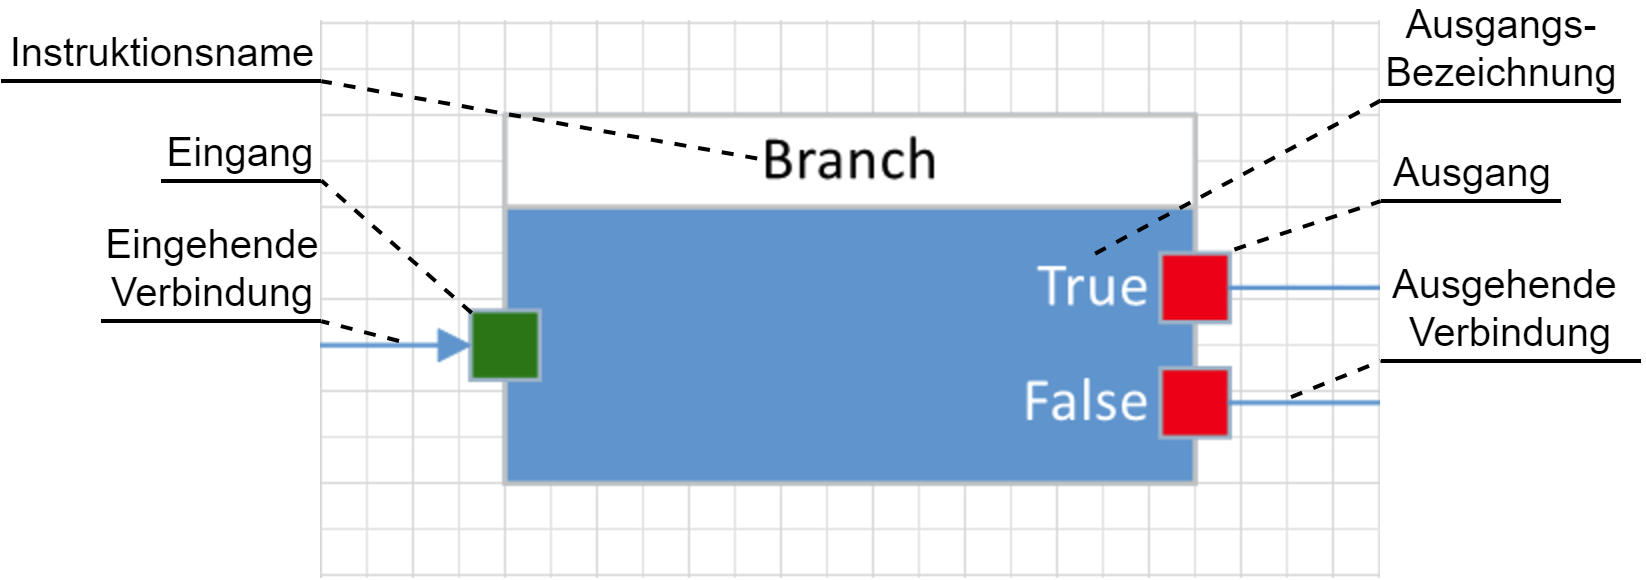
\includegraphics[width=0.8\textwidth]{img/SingleNodeWithAnnotations.png}
	\caption[Beschriftung einer DSL-Instruktion]{Eine einzelne Instruktion wie sie (ohne die Beschriftung) in einem Konversationsrouting dargestellt wird. Abgebildet ist die Branch-Instruktion, welche über einen Eingang und zwei Ausgänge verfügt. Die If-Bedingung, welche den zu nehmenden Ausgang bestimmt, ist nicht in der Instruktion dargestellt, sondern wird auf als Eigenschaft in einem separaten Fenster der Benutzeroberfläche konfiguriert.}
	\label{fig:SingleNode}
\end{figure}

\subsection{Beispiel}
Ein Beispiel soll im Folgenden die Anwendung der domänenspezifischen Sprache näher veranschaulichen. In Abbildung \ref{fig:ExampleRouting} ist ein Konversationsrouting durch ein Modell der DSL spezifiziert. Hier wird für den eingehenden Anruf zu erst eine Fallunterscheidung durchgeführt: Mittels eines C\#-Ausdrucks (dargestellt in der Abbildung durch einen Code-Editor), der per System-Aufruf den aktuellen Wochentag ermittelt, wird entschieden, ob das Routing an einem Sonntag ausgeführt wird. Ist dies der Fall, wird der Ruf terminiert, da es sich um einen Ruhetag handelt. Andernfalls wird eine DTMF-Abfrage gestartet, bei der dem Anrufer in einer abgespielten Audiodatei ein Menü vorgelesen wird. Braucht der Benutzer zu lange, um eine Eingabe zu machen, wird der Timeout-Ausgang gewählt, welcher wieder zurück in die DTMF-Abfrage führt. Bis der Anrufer also eine Eingabe macht oder auflegt, befindet er sich in einer Endlosschleife. Wählt er eine Eins, wird er an ein direktes Ziel weitergeleitet. Wählt er dagegen eine Null, wird eine Hintergrundmusik gestartet und er wird in die Warteschlange eingereiht. Nun verbleibt der Anrufer solange in der Warteschleife, bis er auflegt oder ein Agent seinen Anruf entgegennimmt.  

\begin{figure} %[hbtp]
	\centering
		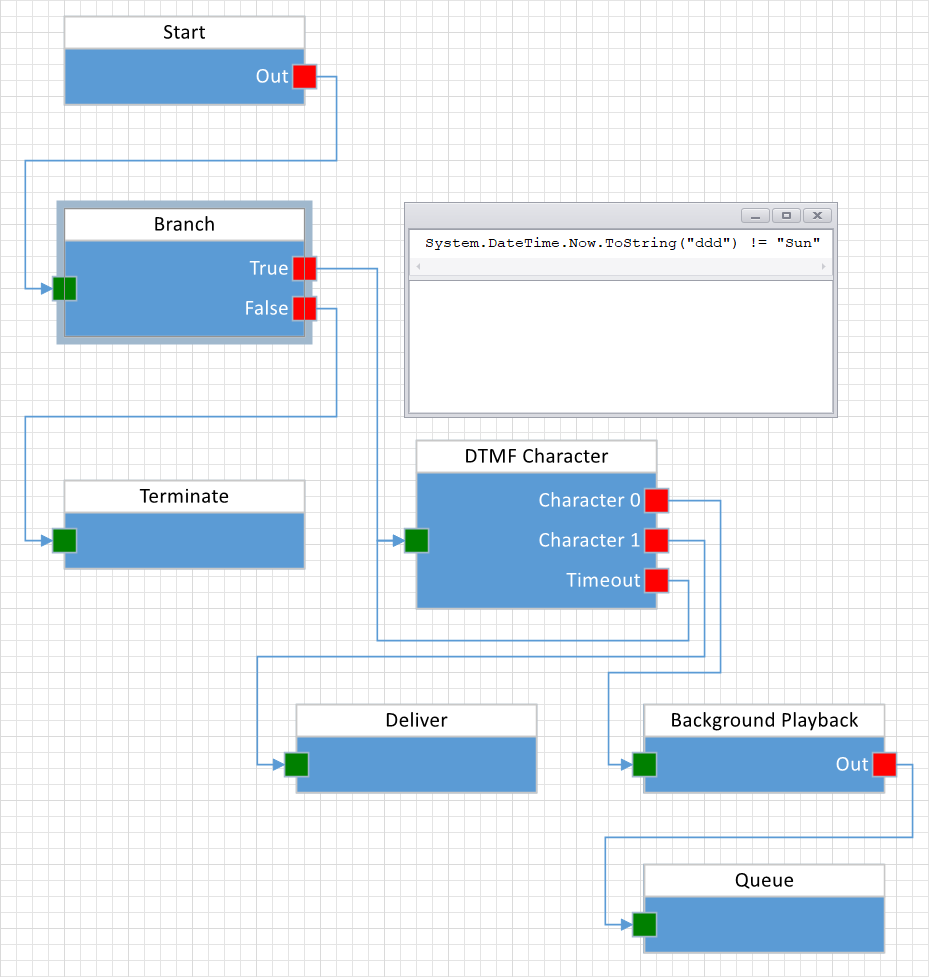
\includegraphics[width=0.79\textwidth]{img/ExampleRoutingRaw.png}
	\caption[Beispiel für ein Konversationsrouting]{Ein beispielhaftes Konversationsrouting}
	\label{fig:ExampleRouting}
\end{figure}

\section{Sprachelemente}
\label{sec:Sprachelemente}
Die Hauptelemente der DSL sind ihre Instruktionen und die Verbindungen zwischen diesen. Auf welche einzelnen Instruktionen der Benutzer Zugriff hat und wie diese spezifiziert sind, ist im Folgenden beschrieben. 

\subsection{Start}
\begin{labeling}{Anzahl Ausgänge}
\item [Eingang] Nein
\item [Anzahl Ausgänge] 1
\item [Parameter] keine
\item [Beschreibung] Der Start-Knoten ist der Anfangspunkt eines Konversationsroutings. Der Programmfluss erreicht diese Instruktion, wenn ein eingehender Anruf von der Routing Engine angenommen wurde. Der Start-Knoten interagiert selbst nicht mit dem Anruf, sondern führt unmittelbar die im Ablauf vorgesehene folgende Instruktion aus. Die Start-Instruktion muss in jedem DSL-Modell vorhanden sein und ist ein notwendiges Kriterium für eine erfolgreiche Validierung des Modells. 
\end{labeling}

\subsection{Media Playback}
\label{subsec:Media Playback}
\begin{labeling}{Anzahl Ausgänge}
\item [Eingang] Ja
\item [Anzahl Ausgänge] 1
\item [Parameter] Die abzuspielende Audiodatei
\item [Beschreibung] Der Media Playback-Knoten kann vom Benutzer verwendet werden, um Audiodateien abzuspielen. Denkbare Anwendungsfälle sind das Abspielen von Begrüßungsansagen oder Musik-Einspieler. Der Kontrollfluss des Konversationsroutings hält solange bei dieser Instruktion an, wie die Audiodatei dauert und wird erst nach dem Abspielen fortgeführt.  Die abzuspielende Audiodatei muss über die Administration von MyContactCenter vor der Auswahl über einen eigenen Dialog eingespielt werden und wird nach Sprache und Wissensgebiet kategorisiert. Auf diese Weise kann mit dem gleichen Media Playback-Knoten für eine Konversation, die beispielsweise als Englisch kategorisiert ist, eine englische Ansage abgespielt werden während für eine spanische Konversation eine entsprechend spanische Audiodatei abgespielt wird.
\end{labeling}

\subsection{Background Playback}
\begin{labeling}{Anzahl Ausgänge}
\item [Eingang] Ja
\item [Anzahl Ausgänge] 1
\item [Parameter] Die abzuspielende Audiodatei
\item [Beschreibung] Ähnlich wie Instruktion aus Abschnitt \ref{subsec:Media Playback} wird auch bei der Background Playback-Instruktion eine Audiodatei abgespielt. Im Gegensatz zu Media Playback blockiert Background Playback jedoch nicht: Das Konversationsrouting wird mit der nächsten Instruktion fortgeführt. Die abgespielte Audiodatei wird in einer Schleife und im Falle einer weiteren Audiowiedergabe mit geringerer Lautstärke abgespielt. Wird der Ruf an einen Agenten zugestellt wird jegliche Background Playback-Wiedergabe beendet. Background Playback ist vor allem dafür vorgesehen, Hintergrundmusik und Ähnliches abzuspielen.
\end{labeling}

\subsection{DTMF Character}
\begin{labeling}{Anzahl Ausgänge}
\item [Eingang] Ja
\item [Anzahl Ausgänge] 13
\item [Parameter] \begin{itemize} \item Eine abzuspielende Audiodatei  \item Dauer des Eingabezeitfensters in Millisekunden \end{itemize}
\item [Beschreibung] Das Mehrfrequenzwahlverfahren (engl. Dual-tone multi-frequency signaling, kurz DTMF) ist eine aus der analogen Telefontechnik stammende Technologie zur Abfrage von Benutzereingaben über eine Telefontastatur. Das Verfahren ist auf 16 Symbole beschränkt, die mit einer Telefontastatur abgedeckt werden können: Die Zahlen von null bis neun, die Buchstaben A bis D, sowie die Raute und der Asterisk (vgl. \cite{Durda:06}). DTMF ist auch im Session Initiation Protocol implementiert und kann in Konversationsroutings mit der DTMF Character-Instruktion benutzt werden. Wenn der Kontrollfluss auf diesen Knoten trifft, wartet das Routing für das per Parameter vorgesehene Zeitfenster ab, bevor die nächste Instruktion ausgeführt wird. Gibt der Anrufer in dieser Zeit eine Eingabe über seine Telefontastatur ein, wird einer von zwölf Ausgängen gewählt, dessen Bezeichner mit der eingegebenen Taste übereinstimmt. Die zwölf Ausgänge bilden die Ziffern 0 bis 9, die Raute und den Asterisk ab. Die Buchstaben A bis D wurden für die Instruktion ausgelassen, da diese Symbole für typische Anrufer, welche meistens eine Standard-Telefontastatur benutzen, nicht relevant sind. Der dreizehnte mit ``Timeout'' bezeichnete Ausgang wird gewählt, wenn die Zeit des Eingabezeitfenster verstrichen ist und der Benutzer in dieser Zeit keine Eingabe getätigt hat. Zusätzlich ist eine Audiodatei spezifizierbar, welche während des Eingabezeitfensters abgespielt wird.  
\end{labeling}

\subsection{Set Skill}
\label{subsec:Set Skill}
\begin{labeling}{Anzahl Ausgänge}
\item [Eingang] Ja
\item [Anzahl Ausgänge] 1
\item [Parameter] Der zu setzende Wissensbereich
\item [Beschreibung] Damit die automatische Kontaktverteilung von MyContactCenter funktioniert, müssen Konversationen in Sprachen (engl. languages) und Wissensbereiche (engl. Skills) eingeteilt werden. Die Kategorisierung dieser Konversationen ist auch innerhalb eines Konversationsroutings möglich. Dazu dient die Set Skill-Instruktion, welche der Konversation ein dem System bekannten Wissensbereich zuweist. Der Benutzer kann so aus einer Liste der verfügbaren Wissensbereiche einen Bereich wählen, in den die aktuelle Konversation passt.
\end{labeling}

\subsection{Set Language}
\label{subsec:Set Language}
\begin{labeling}{Anzahl Ausgänge}
\item [Eingang] Ja
\item [Anzahl Ausgänge] 1
\item [Parameter] Die zu setzende Sprache
\item [Beschreibung] Verhält sich für Spachen analog zur Instruktion aus \ref{subsec:Set Skill}.
\end{labeling}

\subsection{Branch}
\begin{labeling}{Anzahl Ausgänge}
\item [Eingang] Ja
\item [Anzahl Ausgänge] 2
\item [Parameter] Ein C\#-Ausdruck der bei Auswertung einen booleschen Wert zurückgibt
\item [Beschreibung] Verzweigungen im Konversationsrouting machen es dem Benutzer möglich, komplexere Abläufe durch Fallunterscheidungen zu modellieren und so mehr Anwendungsszenarien für das Konversationsrouting abzubilden. Solche Verzweigungen werden durch die  Branch-Instruktion möglich. Diese besitzt als Parameter einen frei programmierbaren C\#-Ausdruck, welcher als Boolean auswertbar sein muss. Bei Ausführung einer Branch-Instruktion wird der Ausdruck ausgewertet und je nach Ergebnis einer der beiden mit ``True'' und ``False'' bezeichneten  Ausgänge für die folgende Instruktion ausgewählt.
\end{labeling}

\subsection{Script}
\label{subsec:Script}
\begin{labeling}{Anzahl Ausgänge}
\item [Eingang] Ja
\item [Anzahl Ausgänge] Variabel
\item [Parameter] C\#-Quellcode
\item [Beschreibung] Ein Ziel der domänenspezifischen Sprache ist zwar, dem Benutzer das langwierige Programmieren mit einer Universalsprache zu ersparen. Aber auf diese Weise können nicht alle relevanten Anwendungsfälle abgedeckt werden. In den Fällen, in denen die Sammlung an grundlegenden Instruktionen nicht ausreicht, wird es dem Benutzer ermöglicht, mittels der Script-Instruktion eigenen C\#-Code im Zuge eines Konversationsroutings auszuführen. Der Skript-Code wird direkt als Parameter der Instruktion übergeben und unterliegt gewissen Rahmen-Bedingungen. Es wird nur Code zugelassen, der laut den C\#-Vorschriften in einem Methoden-Körper möglich ist. Damit entfallen Operationen wie das Definieren von eigenen Typen oder Funktionen. Ebenfalls wird vom Benutzer verlangt, am Ende seines Skripts einen String zurückzuliefern. Dieser String muss identisch mit dem Bezeichner eines der Ausgänge der Skript-Instruktion sein, deren Anzahl und Bezeichner durch den Benutzer festgelegt werden. Auf diese Weise hat der Benutzer innerhalb seines C\#-Skripts die Kontrolle darüber, welcher Ausgang und somit welche Instruktion als nächstes im Konversationsrouting ausgeführt werden. Für eine erfolgreiche Validierung eines Modells muss jeglicher vom Benutzer geschriebene Code compilierbar sein.   
\end{labeling}

\subsection{Deliver}
\label{subsec:Deliver}
\begin{labeling}{Anzahl Ausgänge}
\item [Eingang] Ja
\item [Anzahl Ausgänge] Keine
\item [Parameter] Sip-Uri des Zustellungsziels
\item [Beschreibung] Ein möglicher Endpunkt in einem Konversationsrouting ist die Zustellung an einen Sip User Agent, zum Beispiel einen MyCC-Agenten. Dies wird mit dem Deliver-Knoten erreicht, welcher als Parameter einen United Resource Identifier (URI) als String erhält. URIs werden in SIP zur Identifizierung von User Agents benutzt. Der aktuelle Kontrollfluss des Konversationsroutings gibt an dieser Stelle die Kontrolle über die Konversation an den spezifizierten Teilnehmer ab. Daher besitzt die Deliver-Instruktion keinen Ausgang, mit dem man eine unmittelbare Nachfolgeinstruktion angeben könnte.
\end{labeling}

\subsection{Queue}
\label{subsec:Queue}
\begin{labeling}{Anzahl Ausgänge}
\item [Eingang] Ja
\item [Anzahl Ausgänge] Keine
\item [Parameter] Keine
\item [Beschreibung] Neben der direkten Zustellung an einen Agenten kann ein Anruf auch in der Warteschlange platziert werden, welche dann die automatische Verteilung an einen freien Agenten übernimmt. Dies kann über die Queue-Instruktion erreicht werden. Warteschlangen sind nach Sprache und Wissensbereich kategorisiert und beim Ausführen der Queue-Anweisung wird der eingehende Anruf entsprechend der aktuell eingestellten Sprache und des aktuellen Wissensbereich (siehe Instruktionen \ref{subsec:Set Language} und \ref{subsec:Set Skill}) in eine passende Warteschlange einsortiert. Ist ein Agent bereit den Anruf anzunehmen, wird dieser zu ihm durchgestellt.
\end{labeling}

\subsection{Terminate}
\begin{labeling}{Anzahl Ausgänge}
\item [Eingang] Ja
\item [Anzahl Ausgänge] Keine
\item [Parameter] Grund der Terminierung
\item [Beschreibung] Die Terminate-Instruktion ermöglicht das kontrollierte Beenden des Anrufs durch die Routing Engine. Ähnlich wie die Deliver-Instruktion aus Abschnitt \ref{subsec:Deliver} ist auch die Terminate-Instruktion ein Konversationsroutingendpunkt und besitzt daher keine Ausgänge. Als Parameter nimmt Terminate einen Grund für das Beenden des Rufs entgegen. Der Grund kann aus einer Aufzählung von vordefinierten Anlässen ausgewählt werden.
\end{labeling}

\subsection{Variablen}
\label{subsec:Variablen}
Variablen unterstützen den Benutzer beim Schreiben von eigenem C\#-Code, wie zum Beispiel in Script- oder Branch-Knoten. Variablen können vom Benutzer deklariert werden und sind nicht für eine einzelne Instruktion angelegt, sondern auf Ebene des Konversationsroutings definiert. Sie erscheinen nicht als Rechteck in der Notation wie andere Instruktionen, sondern sind über Dialoge in der grafischen Benutzeroberfläche konfigurierbar. Eine deklarierte Variable kann überall dort im Routing verwendet werden, wo der Benutzer eigenen C\#-Code schreibt. Zur Auswahl für den Variablentyp stehen die primitiven Datentypen int, float, double, bool, string und zusätzlich zur Abbildung von Daten und Zeitpunkten der Typ DateTime aus dem Standard C\#-Namespace zur Verfügung. Zusätzlich zum Typ muss der Benutzer einen Bezeichner angeben, unter dem die Variable im Konversationsrouting referenziert werden kann. Der Wert einer Variable kann mit der Set Variable-Instruktion gesetzt werden, die in Abschnitt \ref{subsec:Set Variables} erläutert wird. 

\subsection{Funktionen}
Zusätzlich zu Variablen kann der Benutzer eigene Funktionen deklarieren, welche ebenfalls in C\# definiert werden. Ähnlich wie Variablen sind Funktionsdeklarationen keine Instruktion, die in der Notation als Rechteck symbolisiert sind, sondern Eigenschaften des Routings. Sie werden daher auch über gesonderte Dialoge der grafischen Benutzeroberfläche angelegt. Für eine Funktionsdeklaration gibt der Benutzer den Bezeichner, eine Liste von Parametern mit Typ und Bezeichner, den Rückgabetyp und den Funktionskörper an. Für alle Typen steht die gleiche Auswahl, die auch bei Variablen angeboten wird, zur Verfügung. Beim Rückgabetyp kann der Benutzer zusätzlich void angeben, um eine Funktion ohne Rückgabe zu definieren. Ist eine Funktion deklariert, kann sie im gesamten Konfigurationsrouting dort aufgerufen werden, wo der Benutzer eigenen C\#-Code angibt.  

\subsection{Set Variables}
\label{subsec:Set Variables}
\begin{labeling}{Anzahl Ausgänge}
\item [Eingang] Ja
\item [Anzahl Ausgänge] 1
\item [Parameter] Eine Sammlung an Variablenzuweisungen
\item [Beschreibung] Wie in \ref{subsec:Variablen} beschrieben, werden Variablen-Deklarationen auf Ebene des Konversationsroutings vollzogen und treten nicht als konkrete Instruktion in der grafischen Notation in Erscheinung. Wert-Zuweisungen werden jedoch mittels der Set Variables-Instruktion umgesetzt. Hier kann der Benutzer eine Liste von Zuweisungen hinterlegen. Jede Zuweisung enthält eine Variable aus der Liste der Deklarationen und einen frei programmierbaren C\#-Ausdruck. Führt der Programmfluss die Set Variables-Instruktion aus, werden die Wertzuweisungen ausgeführt.
\end{labeling}

\subsection{Vordefinierte Variablen}
Neben den selbst angelegten Variablen hat der Benutzer in seinen Scripten auch Zugriff auf Variablen, die schon von der DSL vorgegeben sind. Dies sind die Variablen Skill und Language, welche jeweils als String verfügbar sind. Diese kann der Benutzer in seinem eigenen Code auslesen, oder setzen. In letzterem Fall wird so die gleiche Funktion erfüllt, die sonst die Instruktionen aus Abschnitt \ref{subsec:Set Skill} und \ref{subsec:Set Language} übernehmen. Setzt der Benutzer die Sprache auf oder den Wissensbereich auf einen Wert, der nicht existiert, wird die Variable nicht verändert. 

\section{Verarbeitungsschritte}
\label{sec:Verarbeitungsschritte}
Zwischen der Modellierung und der letztendlichen Ausführung eines DSL-Modells finden sieben Verarbeitungsschritte statt. Abbildung \ref{fig:Verarbeitungsschritte} veranschaulicht den Vorgang, den ein Konversationsrouting von der Spezifikation bis zur Ausführung durchläuft. Am Anfang steht die Modellierung durch den Benutzer. Hier werden die Instruktionen in einem oben beschriebenen Graphen angeordnet und Verbindungen gezogen, um einen Konversationsroutingablauf zu spezifizieren. Intern und für den Benutzer unsichtbar wird im Editor synchron zu der graphischen Repräsentation eine C\#-Datenstruktur erstellt, welche die abstrakte Syntax als .NET Objekt abbildet. Diese Struktur wird beim Abspeichern des Modells im Protobuf-Format serialisiert und in einer Datenbank abgespeichert. Die serialisierten Daten werden von der Routing Engine abgerufen und deserialisiert. Das Resultat ist das vom Benutzer angelegte C\#-Objekt. Die Struktur wird an den Transformator übergeben, welcher diese in abstrakte MSIL-Syntax umwandelt. Laut \cite[S. 72f]{Kleppe:09} handelt es sich dabei um eine strukturelle Transformation (engl. structural Transformation), da von der abstrakten Syntax der DSL in die abstrakte Syntax der Common Intermediate Language übersetzt wird. Die Routing Engine kompiliert die MSIL-Syntax nun im Arbeitsspeicher mit der Hilfe von Roslyn, und erhält eine .NET-Assembly. Der Code in dieser Assembly wird anschließend für jeden eingehenden Anruf ausgeführt. 

\begin{figure} %[hbtp]
	\centering
		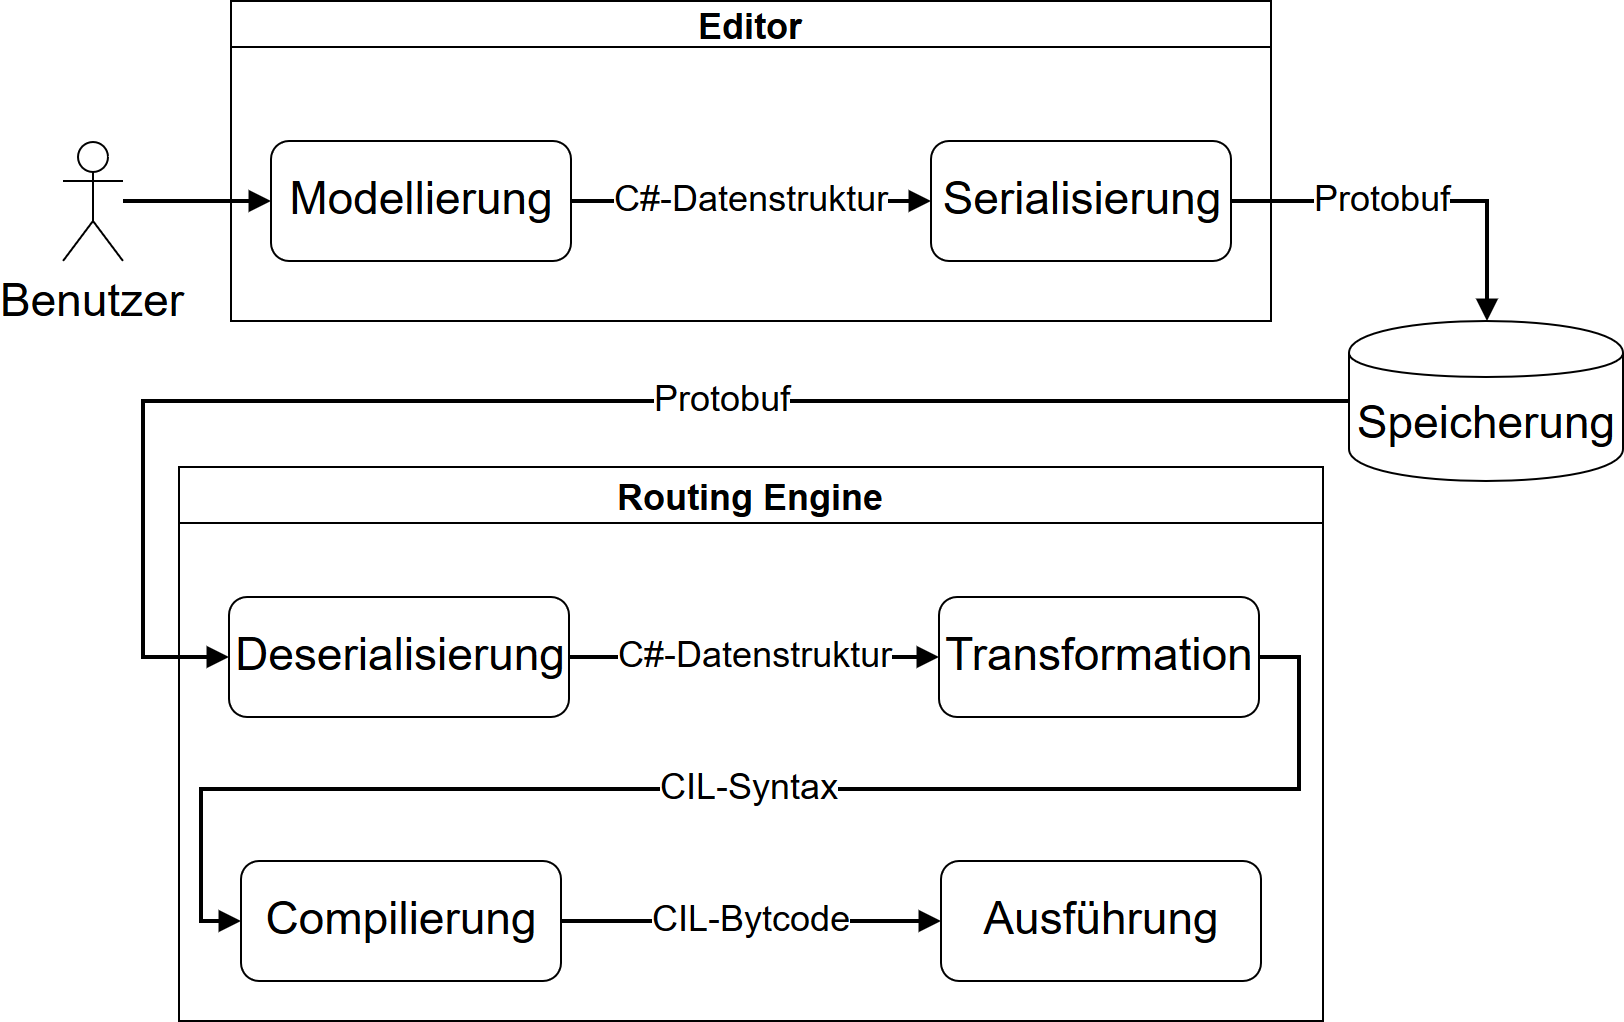
\includegraphics[width=\textwidth]{img/Verarbeitungsschritte.png}
	\caption[Verarbeitungsschritte eines DSL-Modells]{Die Verarbeitungsschritte eines DSL-Modells schematisch dargestellt. Die Schritte sind als abgerundete Rechtecke dargestellt, deren zeitliche Abfolge durch Pfeile gezeigt wird. Die Pfeile sind mit der Eingabe für den jeweils nächsten Verarbeitungsschritt beschriftet. Die Container zeigen an, im Zuge welches Programmcodes die Verarbeitungsschritte ausgeführt werden. Zuerst modelliert der Benutzer einen Ablauf im Editor. Anschließend wird das Modell dort serialisiert und in einer Datenbank abgespeichert. Nach der Deserialisierung in der Routingengine wird das Modell dort transformiert, kompiliert und ausgeführt.}
	\label{fig:Verarbeitungsschritte}
\end{figure}
\chapter{Implementierung}
\label{chap:Implementierung}

\section{Editor}
\label{sec:Editor}
Der Editor ist die Schnittstelle zwischen der DSL und einem menschlichen Benutzer. Hier wird ein DSL-Modell durch Interaktion mit der konkreten Syntax erstellt oder bearbeitet. Die konkrete Syntax nimmt die Form eines Graphen an, der in Kapitel \ref{chap:Einleitung} beschrieben ist. Mit dem Editor kann dieser Graph über die grafische Benutzeroberfläche in die gewünschte Form gebracht werden. Abbildung \ref{fig:EditorGUI} zeigt und erklärt die Komponenten der grafischen Benutzeroberfläche.
\newline 
Neben der Interaktion mit dem Benutzer ist die andere Aufgabe des Editors, die konkrete Syntax in abstrakte Syntax umzuwandeln. Während der Benutzer über die grafische Benutzeroberfläche mit der konkreten Syntax interagiert, also Instruktionen hinzufügt und Verbindungen zieht, wird Editor-intern die für den Benutzer unsichtbare abstrakte Syntax geformt. Die abstrakte Syntax ist durch die Instanz einer C\#-Datenstruktur repräsentiert, welche für die weiteren Verarbeitungsschritte gespeichert wird (siehe Abschnitt \ref{sec:Verarbeitungsschritte}). In der Literatur wird die Datenstruktur, welche die abstrakte Syntax beinhaltet, auch semantisches Modell (engl. semantic model)\cite[S. 159ff]{Fowler:11}, oder abstraktes Syntax-Modell (engl. abstract syntax model)\cite[S. 78ff]{Kleppe:09} genannt. Der Editor bildet eine vom Benutzer modellierte Instanz der konkreten Syntax auf eine Instanz des semantischen Modells ab. Diese Abbildung ist bidirektional: Änderungen am semantischen Modell spiegelt die grafische Benutzeroberfläche in der konkreten Syntax wider. 
\newline
Der Editor ist als eine Windows Forms-Anwendung umgesetzt und implementiert das Model-View-Viewmodel-Entwicklungsmuster (kurz MVVM). Ähnlich wie bei verwandten Entwurfsmustern wie zum Beispiel Model-View-Controller (MVC) geht es bei MVVM darum, die Darstellung einer Anwendung von ihrer Logik zu trennen. Dies geschieht durch eine Einteilung in drei verschiedene Schichten: Dem View, dem Viewmodel und dem Model. Die View-Schicht dient zur Darstellung der Anwendung und umfasst die Komponenten der grafischen Benutzeroberfläche. Sie erhält die nötigen Daten zur Darstellung vom Viewmodel über sogenannte Datenbindung (engl. Data Binding). Dabei werden Daten über ein Framework an einander gebunden und werden so vom System bei jeder Zustandsänderung synchronisiert. Ändern sich also Daten im Viewmodel wird dies unverzüglich im View angezeigt. Das Viewmodel kümmert sich um die Präsentationslogik. Das heißt es ist dafür zuständig Daten so aufzubereiten, dass diese dem View per Datenbindung zur Verfügung gestellt werden können. Dafür hat das Viewmodel Zugriff auf das Model, welches die Daten speichert. Im Viewmodel wird auch die Geschäftslogik sowie Speicher- und Lade-Aktionen ausgeführt. In .NET wird MVVM vor allem im Zuge der Windows Presentation Foundation eingesetzt, kann aber durch das Devexpress-Framework auch in Windows Forms-Anwendungen benutzt werden. 
\newline
Im grafischen Editor der DSL werden die drei Schichten von MVVM durch verschiedene C\#-Klassen abgebildet, welche im Folgenden erläutert werden.

\begin{figure} %[hbtp]
	\centering
		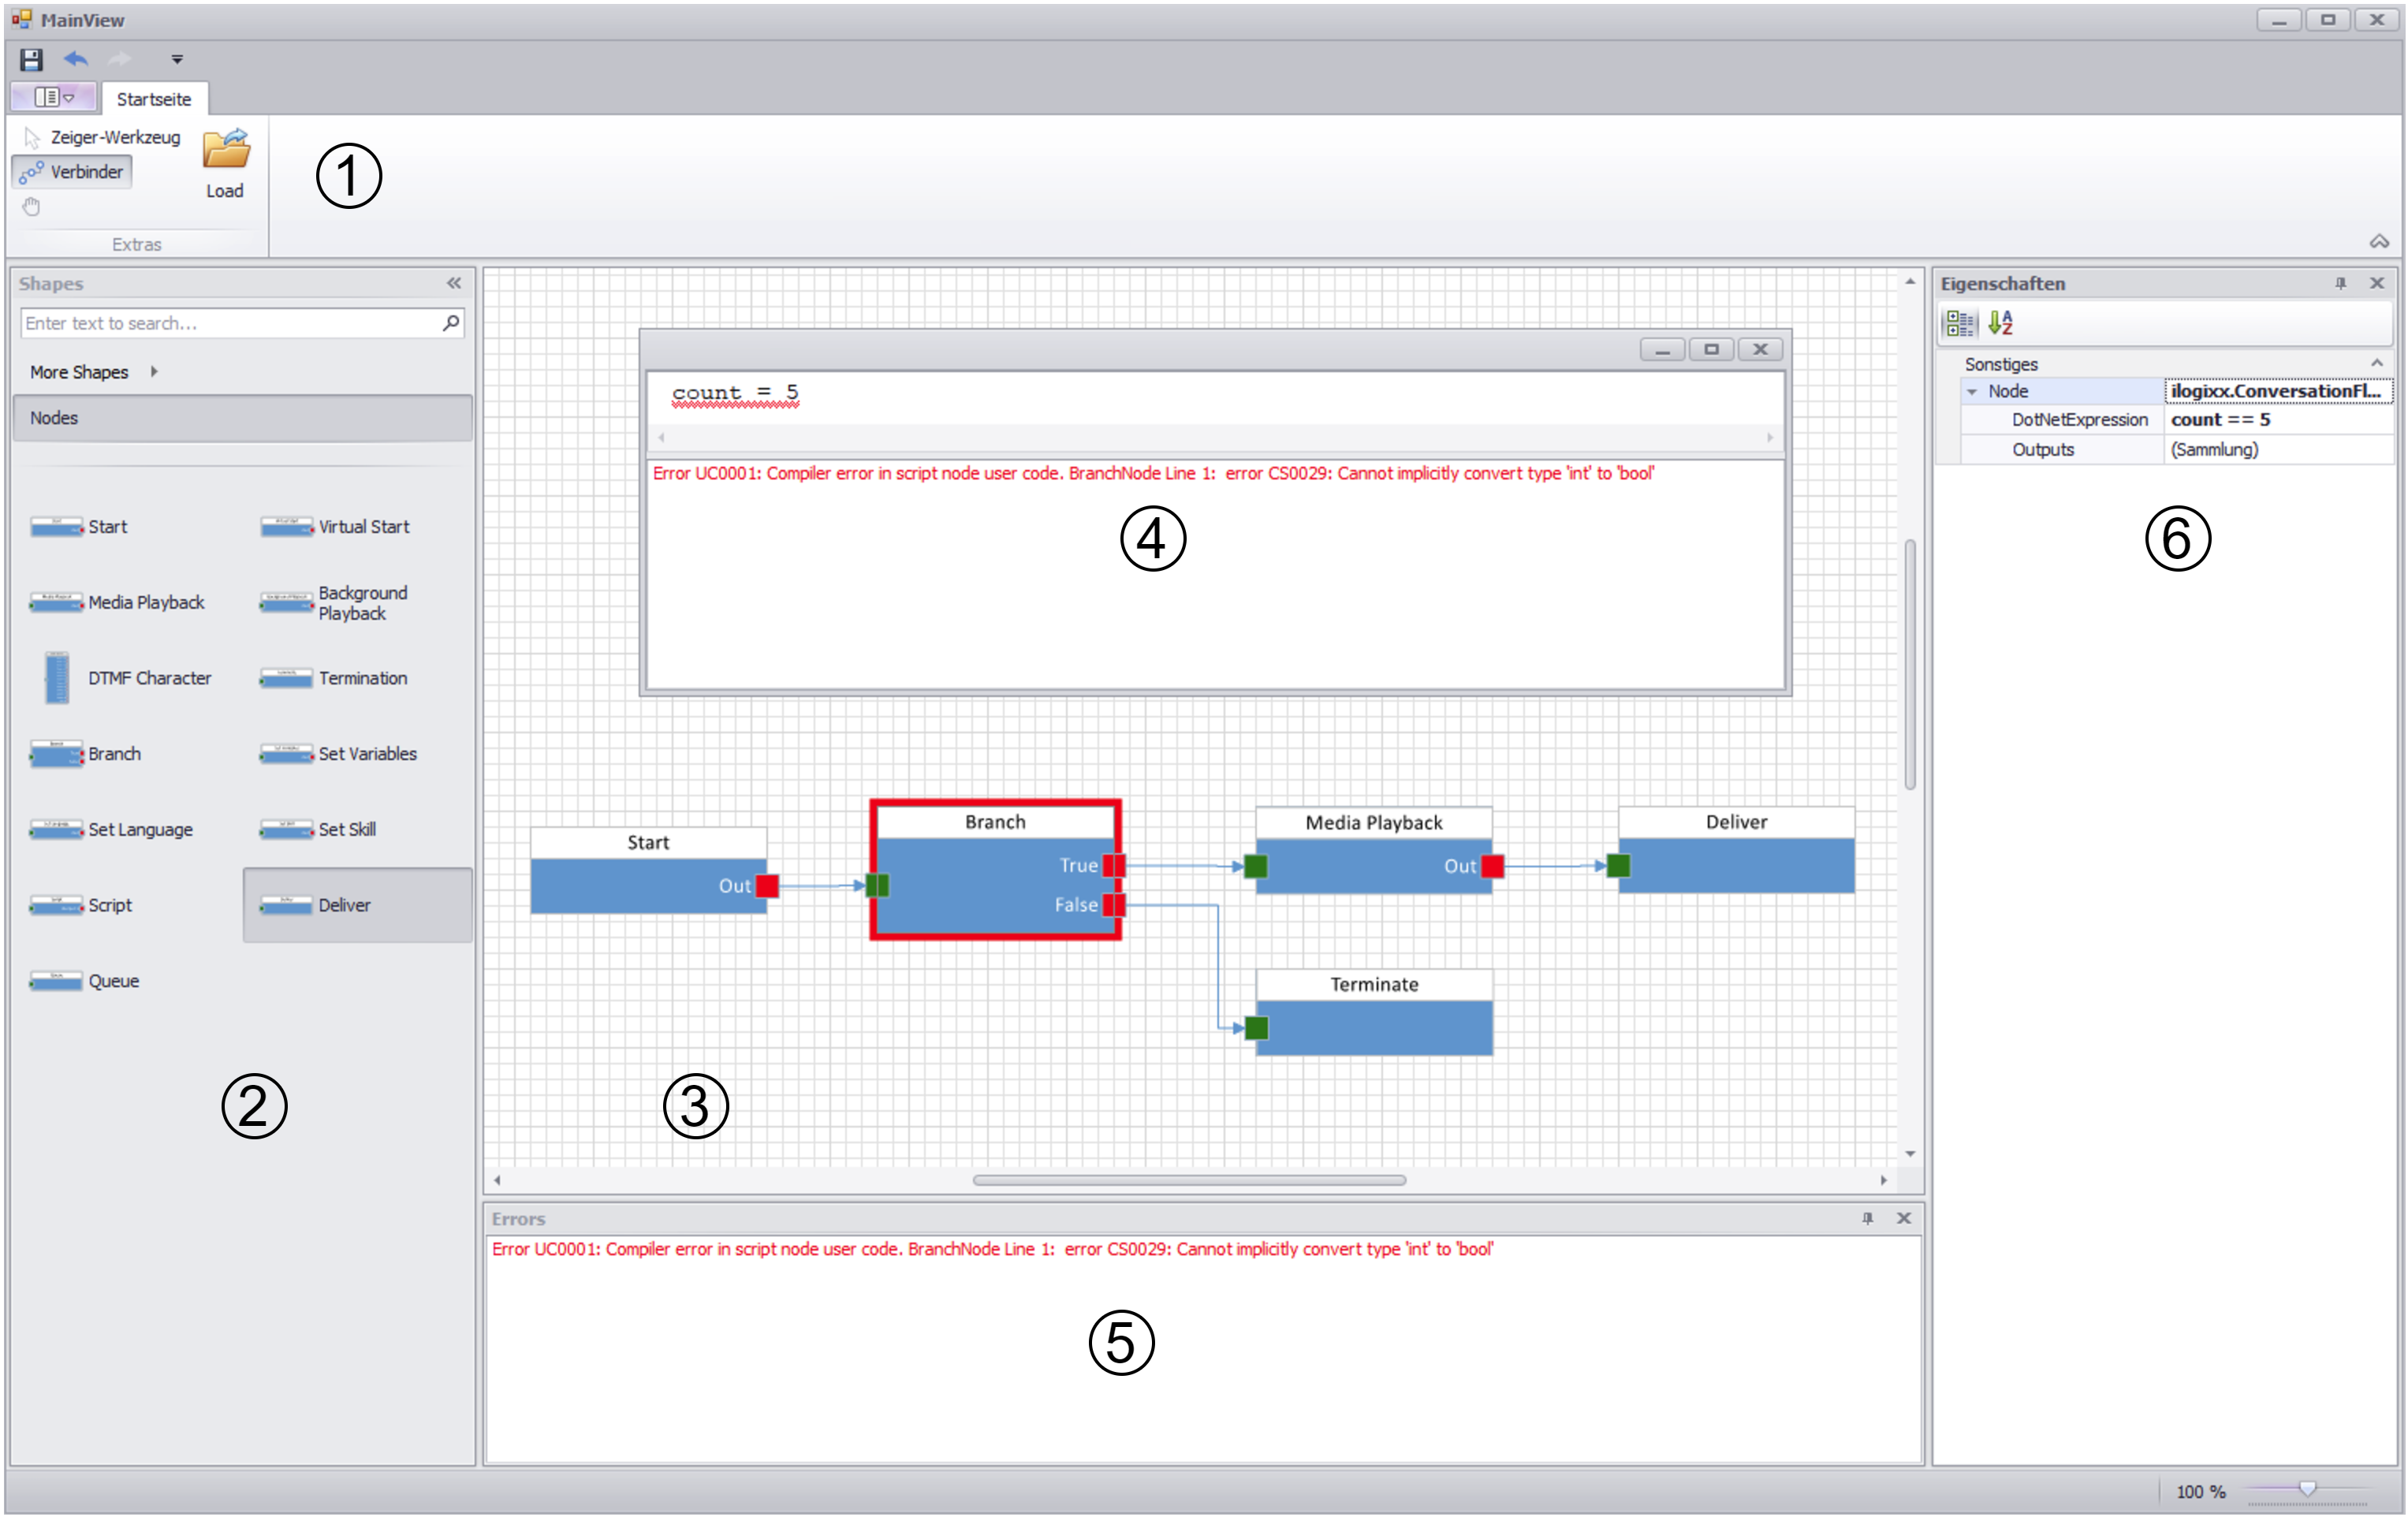
\includegraphics[width=\textwidth]{img/EditorGUI.png}
    \captionsetup{singlelinecheck=off}
	\caption[Die Benutzeroberfläche des Editors]
	{
	\label{fig:EditorGUI}
	Zu sehen ist die Benutzeroberfläche des Editors. Die Nummerierung beziffert folgende Komponenten:
	\begin{enumerate}
	\item Menüleiste. Hier kann der Benutzer Routings speichern oder laden, sowie das Verbindungswerkzeug zum Verbinden von zwei Instruktionen an- und ausschalten.
	\item Instruktionsauswahl-Fenster. Der Benutzer sieht hier eine Übersicht der verfügbaren Instruktionen. Per "Drag and Drop" kann er eine Instruktion auswählen und in das Editor-Fenster ziehen.
	\item Editor-Fenster. Hier kann der Benutzer das Konversationsrouting modellieren, indem er Instruktionen hinzufügt, löscht, anordnet und miteinander verbindet.
	\item Ausdruck-Editor. Der Editor ist in dieser Darstellung stellvertretend für alle Editoren dargestellt, die sich in einem weiteren Fenster öffnen. In diesem Fall ist der Ausdruck-Editor geöffnet, da momentan der boolesche Ausdruck für die Branch-Instruktion editiert wird. Hier kann der Benutzer seinen eigenen Code schreiben. Der Editor verfügt über ein eigenes Diagnose-Fenster, in dem Fehlermeldungen dargestellt werden, die sich auf den zu editierenden Code beziehen.
	\item Diagnose-Fenster. Hier werden alle Fehlermeldungen aufgelistet, die durch die Modell-Validierung detektiert werden. Bei Fehlermeldungen, die sich explizit auf eine Instruktion beziehen, werden diese Instruktionen rot umrandet. Durch einen Doppelklick auf eine Fehlermeldung wird die betroffene Instruktion ausgewählt, oder falls nötig, ein Editor geöffnet der den fehlerhaften Code darstellt.
	\item Parameter-Fenster. Hier können die Parameter der aktuell ausgewählten Instruktion angepasst werden. Ist keine Instruktion ausgewählt, können die weiteren Eigenschaften des Konversationsroutings eingestellt werden, wie zum Beispiel benutzerdefinierte Variablen und Funktionen.
 	\end{enumerate}
 	}
\end{figure}


\subsection[Die Model-Schicht]{Die Model-Schicht: Flow, Node, Input, Output, Connector, Variable, Function}
\label{subsec:Die Model-Schicht}
Die Model-Schicht beinhaltet die C\#-Datenstruktur, welche als semantisches Modell bezeichnet wird. Es handelt sich um das Objekt, welches in der weiteren Verarbeitung die abstrakte Syntax beschreibt. Das semantische Modell selbst weist kein programmatisches Verhalten auf, sondern ist eine reine Datenstruktur. Es besteht aus Instanzen von Klassen, welche die einzelnen Elemente der DSL modellieren und im Namespace ilogixx.ConversationFlow.Core definiert sind. Die Klassenstruktur der Model-Schicht ist in Abbildung \ref{fig:UML:Model-Schicht} als UML-Diagramm aufgeführt.
\newline
Instruktionen werden durch die abstrakte Klasse Node modelliert. Node besitzt eine Liste von Referenzen auf Output-Objekte, welche die Ausgänge einer Instruktion modellieren. Node hat ebenfalls eine Referenz auf ein Objekt vom Typ Input, welches den Eingang eines Knotens symbolisiert. Jede Art von Instruktion hat ihre eigene Subklasse, dargestellt in Abb. \ref{fig:UML:Node-Hierarchy}, welche die Instruktionen aus Abschnitt \ref{sec:Sprachelemente} abbilden. Pro Ausgang einer Instruktion fügt der Konstruktor des entsprechenden Subtypen der Referenzliste der Basisklasse eine neue Referenz vom Typen Output hinzu. Im Konstruktor wird ebenfalls der Input spezifiziert: Hat die Instruktion einen Eingang, wird die Input-Referenz instanziert, andernfalls bleibt sie null. Viele Instruktionen haben die gleiche Anzahl an Ausgängen und einen Eingang. Daher existieren zusätzliche Subtypen, welche die Initialisierungsarbeit übernehmen: Inputnode für Instruktionen, die einen Eingang haben, SingleOutputNode für Instruktionen, die einen einzelnen Ausgang haben und SingleThroughputNode für Instruktionen, die einen Ein- und einen einzelnen Ausgang haben. Alle dreizehn Subtypen für die Instruktionen erben von diesen drei Klassen und passen dort wo nötig ihre Input- und Output-Konfiguration an. Beispielsweise erbt DTMFCharacterNode von InputNode und fügt der Output-Referenzliste dreizehn neue Outputs hinzu.
\newline
Die Klasse Input ist simpel: Sie zeigt über eine Referenz vom Typen Node auf ihre besitzende Instruktion. Die Klasse Output hingegen besitzt einige mehrere Daten. Sie speichert den Bezeichner des Ausgangs als String, einen weiteren String namens DisplayString, welcher vom Benutzer editiert werden kann und auf der Benutzeroberfläche angezeigt wird, einen Boolean namens Visible, welcher bestimmt ob der Ausgang in dem Rechteck der beinhaltenden Instruktion angezeigt wird, und eine Referenz vom Typ Input auf einen Eingang, falls der Ausgang mit einem solchen verbunden sein sollte. Durch letztere Input-Referenz sind die Verbindungen im Konversationsrouting zwischen den Instruktionen implizit gegeben. Zusätzlich existiert eine weitere Klasse namens Connector, welche eine Verbindung explizit definiert. Sie besitzt Referenzen auf diejenigen Input- und die Output-Instanzen, welche in einem Konversationrouting verbunden sind.
\newline
Benutzerdefinierte Variablen und Funktionen sind über die eigenen Klassen Variable und Function abgebildet. Variable besitzt einen Namen vom Typ String und einen Typ, der über einen Enum namens VariableType modelliert ist. Dieser Enum beinhaltet die in \ref{subsec:Variablen} aufgezählten Typen. Function speichert ebenfalls einen Namen vom Typ String und einen Rückgabetyp, welcher über einen Enum mit Namen FunctionReturnType abgebildet ist. Zusätzlich wird der Funktionskörper mit Namen Body als String gespeichert. Die Parameter einer Funktion werden über eine Liste von Referenzen auf Objekte des der eigenen Klasse Parameter modelliert. Ein Parameter besitzt, ähnlich wie die Klasse Variable, einen Namen als String und einen Typ als VariableType. Die Klasse Flow vereint alle oben genannten Klassen: Sie beinhaltet Listen mit Referenzen auf alle Nodes, Connectors, Functions und Variables eines Konversationsroutings. 

\begin{figure} %[hbtp]
	\centering
		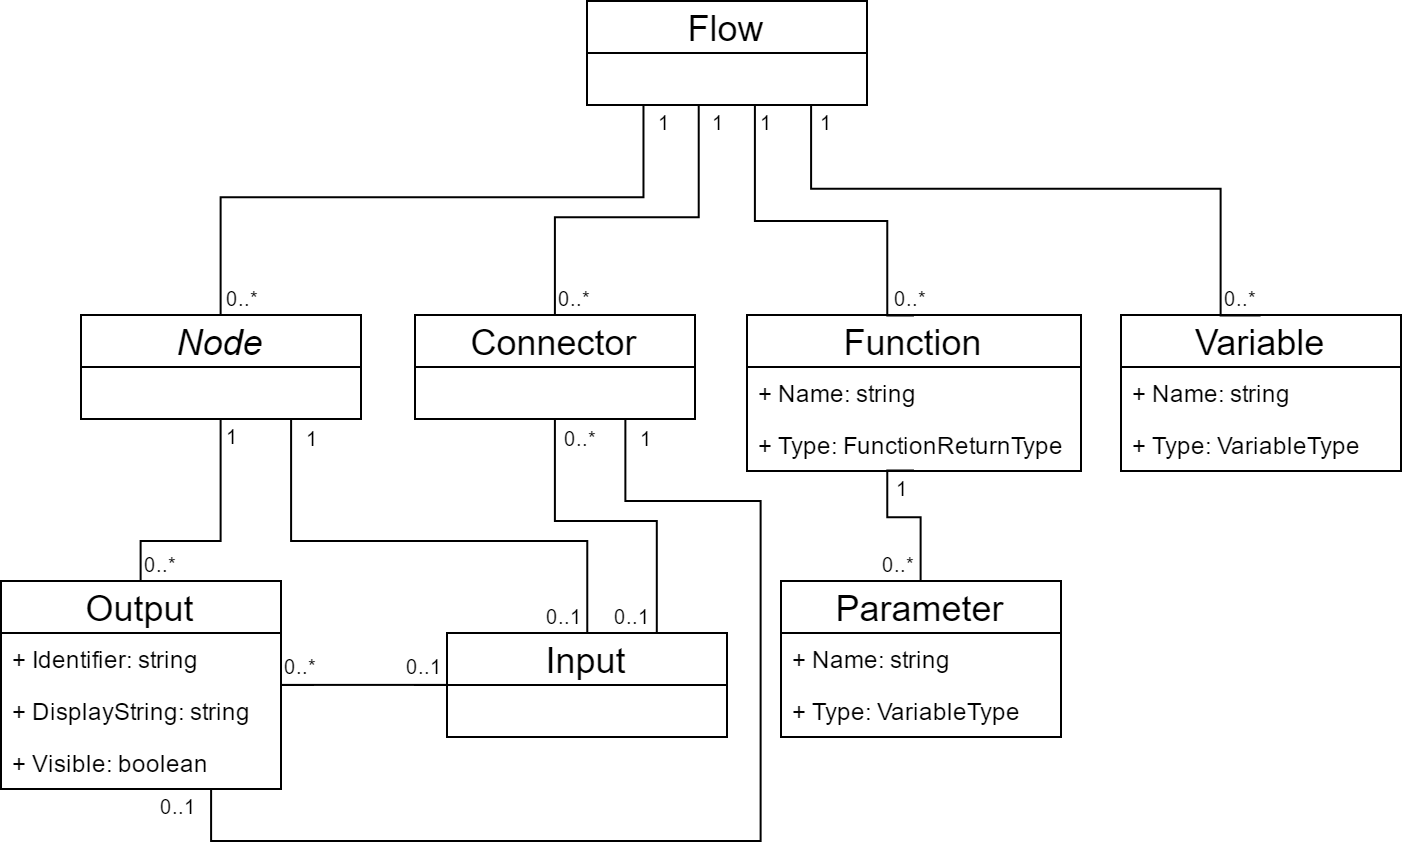
\includegraphics[width=\textwidth]{img/FlowClassStructure.png}
	\caption[Klassenstruktur der Model-Schicht]{Zu sehen ist ein Teil der Klassenstruktur der Model-Schicht. Diese ist zugleich auch das semantische Modell, welches in weiteren Verarbeitungsschritten übergeben wird.}
	\label{fig:UML:Model-Schicht}
\end{figure}

\begin{figure} %[hbtp]
	\centering
		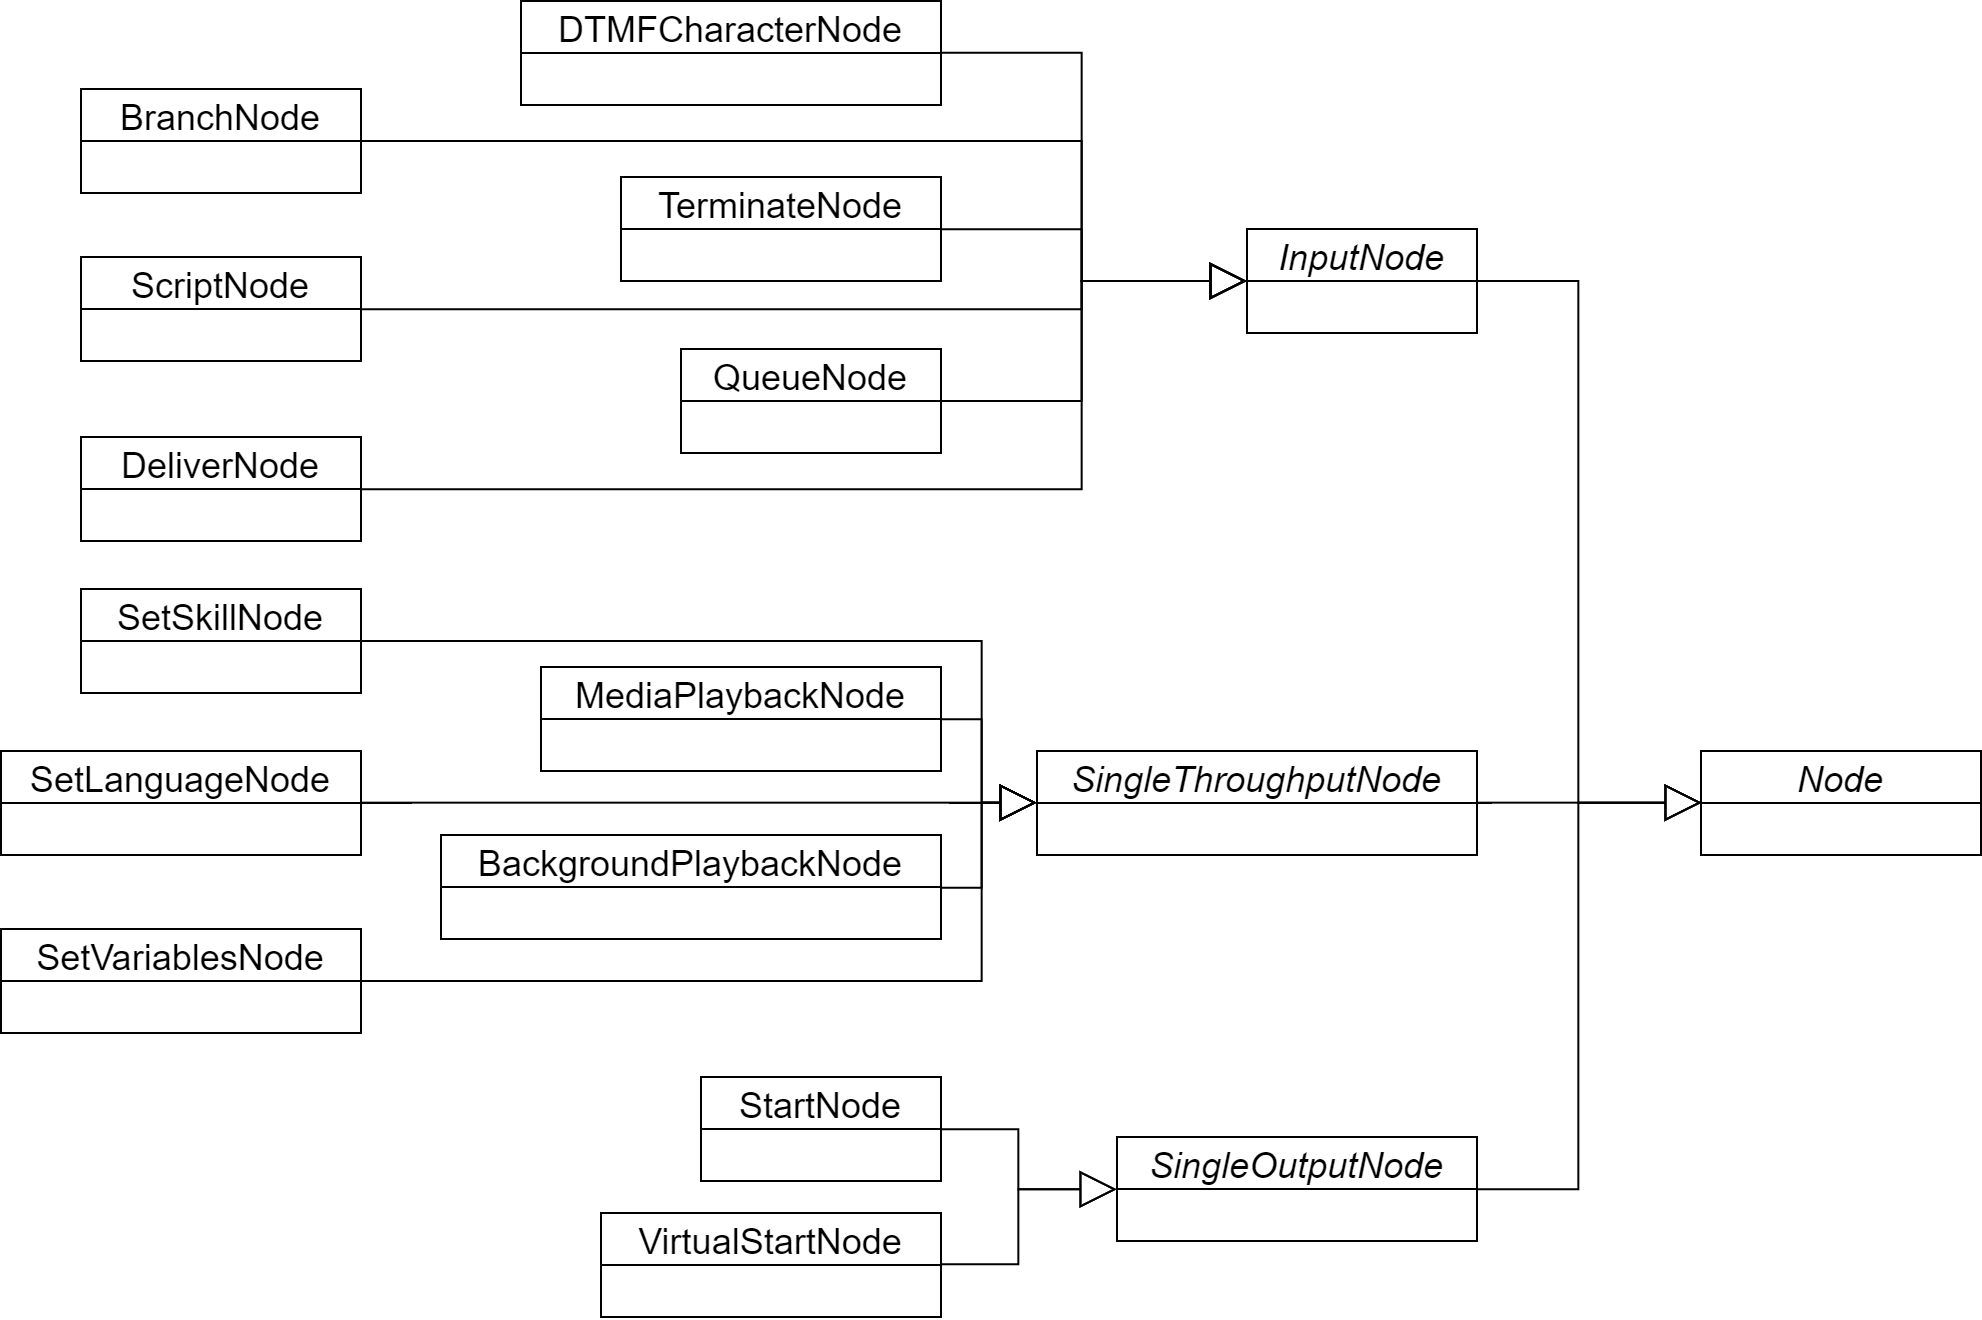
\includegraphics[width=\textwidth]{img/NodeHierarchy.png}
	\caption[Klassenhierarchie der Klasse Node]{Abgebildet ist die Klasse Node und ihre Subtypen. Jede Instruktion der DSL ist durch einen Subtyp von Node abgebildet. Ob die Klasse als Zwischenstufe von InputNode, SingleThroughputNode oder SingleOutputNode erbt, ergibt sich aus der Anzahl an Inputs und Outputs der Instruktion.}
	\label{fig:UML:Node-Hierarchy}
\end{figure}

\subsection[Die Viewmodel-Schicht]{Die Viewmodel-Schicht: FlowDiagramViewmodel, CodeEditorViewModel, FunctionCollectionEditorViewModel}
\label{subsec:Die Viewmodel-Schicht}
In der Viewmodel-Schicht werden die Klasseninstanzen der Model-Schicht so aufbereitet, dass die View-Schicht sie per Datenbindung repräsentieren kann. Die Viewmodel-Schicht reagiert auch auf Eingaben des Benutzers und manipuliert das zu Grunde liegende Model nach dessen Wünschen. Der wichtigste Teil der Viewmodel-Schicht ist in Abbildung \ref{fig:UML:FlowViewModel} dargestellt.  
\newline
Der Hauptbestandteil der Schicht ist die Klasse FlowDiagramViewmodel. Diese besitzt als Member-Variablen Listen auf Referenzen der Model-Komponenten Node, Connector, Variable und Function. Diese Listen sind vom .NET-Typ ObservableCollection, welcher ein Event auslöst, falls Objekte hinzugefügt oder entfernt werden und sind per Devexpress-Datenbindung an die View-Schicht gekoppelt. Das heißt, wenn auf der View-Schicht Elemente des Modells wie zum Beispiel neue Node- oder Connector-Objekte hinzugefügt werden, aktualisieren sich die entsprechenden Listen im FlowDiagramViewmodel. Zusätzlich werden dadurch Events ausgelöst, auf die FlowDiagramViewModel in den Methoden HandleNodesChanged und HandleConnectorsChanged reagiert. Dies wird dazu genutzt, die Referenzen zwischen den Klassen Input und Output aktuell zu halten: Wird ein Connector der Liste hinzugefügt, wird die Input-Referenz des im Connector referenzierten Outputs auf den Input gesetzt, der ebenfalls im Connector verlinkt ist. Der Vorgang wird rückgängig gemacht, wenn ein Connector entfernt wird. Die Datenbindung funktioniert auch umgekehrt: Wenn sich die Input-Referenz eines Outputs ändert, wird ein Event ausgelöst, welches in der Methode HandleOutputPropertyChanged behandelt wird. Dort wird ein neuer Connector mit entsprechenden Input- und Output-Referenzen hinzugefügt. Der grundsätzliche Ablauf der Kommunikation zwischen ViewModel und View ist in Abb. \ref{fig:UML:MVVMSequence} verbildlicht.
\newline 
FlowDiagramViewModel übernimmt mittels der beiden Kommandos WriteToDisk und ReadFromDisk auch das Speichern und Laden von Konversationsroutings. Dafür wird mit den Listen der Node-, Connector-, Variable- und Function-Instanzen ein Flow-Objekt instanziert und mit Protobuf serialisiert. Pfade für die zu schreibenden beziehungsweise lesenden Dateien werden über Dialoge vom Benutzer abgefragt. Die Dialoge werden über vorgefertigte Serviceklassen angezeigt, welche das MVVM-Framework von Devexpress per Dependency Injection zur Verfügung stellt. 
\newline
Einige Instruktionen eines Konversationsroutings benötigen die Möglichkeit, Code einzugeben. Zu diesem Zweck existiert ein weiteres ViewModel, welches dem eingebauten Code-Editor zu Grunde liegt. Das CodeEditorViewModel beinhaltet einen String, welcher den Code enthält. Dieser ist per Datenbindung an den Text des Code-Editors gebunden. Zusätzlich enthält CodeEditorViewModel entweder eine Referenz auf die zu bearbeitende Node, oder die zu bearbeitende Function. Eine Aufgabe des CodeEditorViewmodels ist es, den im Editor eingegebenen Code synchron mit dem Code in der jeweiligen Node oder Function zu halten. 
\newline
Damit der Benutzer die selbst definierten Funktionen verwalten kann, existiert zusätzlich ein Funktions-Editor, in dem neue Funktionen angelegt, gelöscht oder bearbeitet werden können. Für diesen Editor wird ein eigenes ViewModel namens FunctionCollectionViewModel verwendet. Es beinhaltet eine Referenz auf die Liste der Funktionen, die sich im FlowDiagramViewModel befinden und wendet das Ändern, Löschen oder Hinzufügen von Funktionen auf diese Liste an.

\begin{figure} %[hbtp]
	\centering
		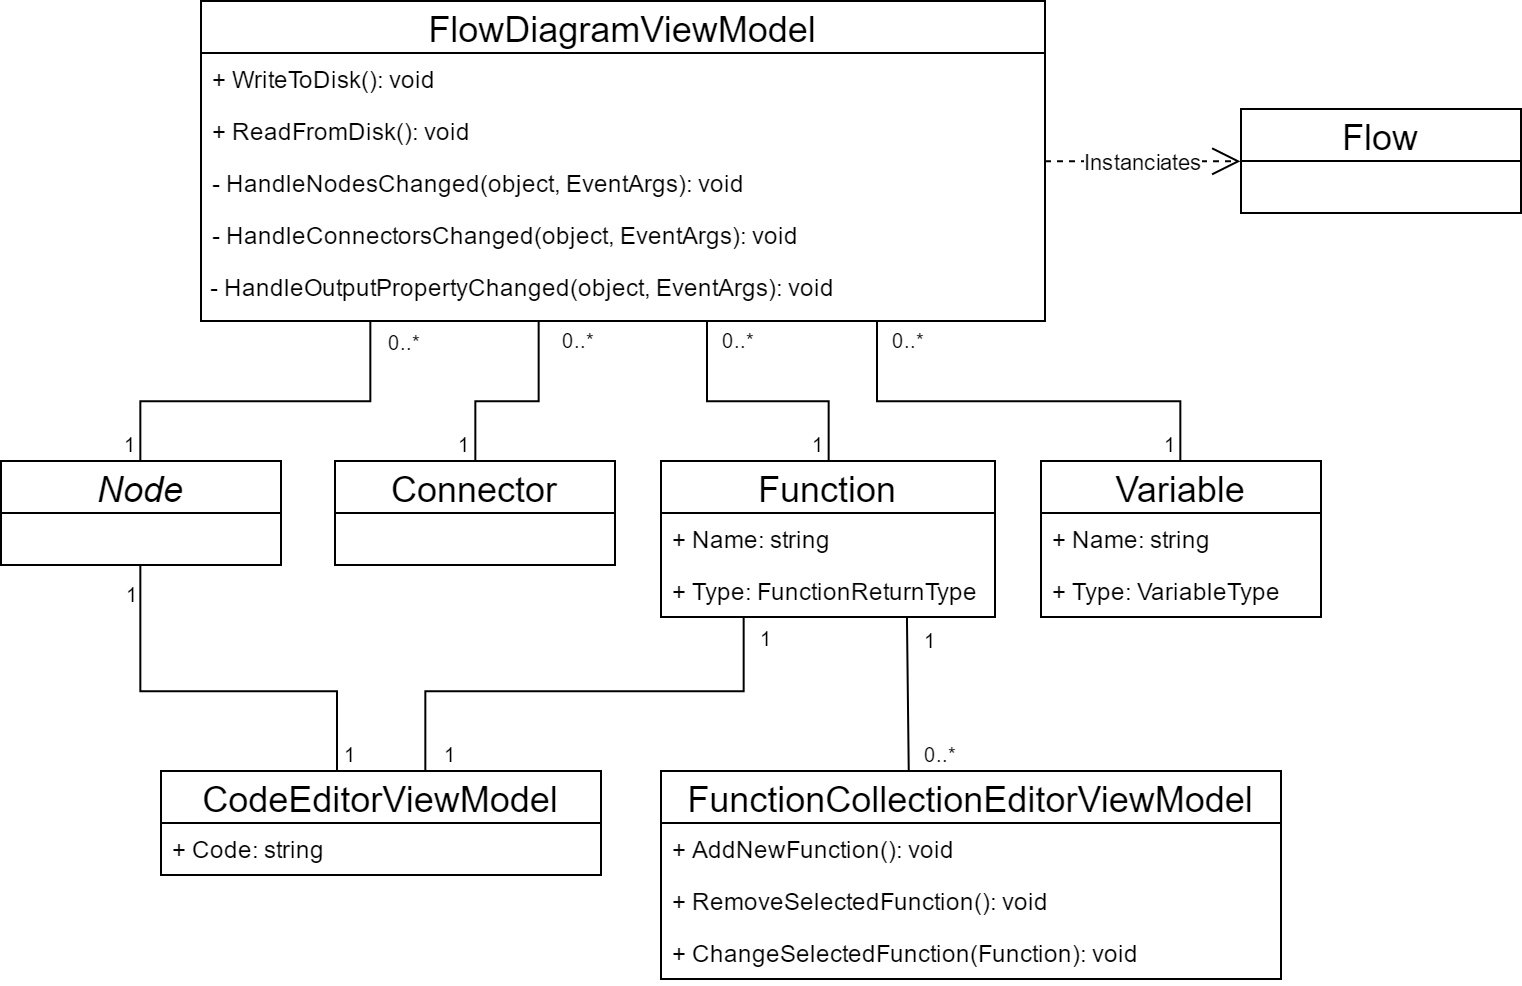
\includegraphics[width=\textwidth]{img/FlowDiagramViewModelUML.png}
	\caption[Klassenstruktur der ViewModelSchicht]{Zu sehen sind die beiden ViewModel FlowDiagramViewModel und CodeEditorViewModel. Ersteres verwaltet Listen mit den Node-, Connector-, Variable- und Function-Instanzen, die beim Instanzieren der Klasse Flow benötigt werden. Letzteres übernimmt die Präsentationslogik für den Code-Editor, indem es Referenzen auf die zu bearbeitenden Node- und Functioninstanzen verwaltet und den Code in Form eines Strings nach für die Datenbindung bereit stellt.}
	\label{fig:UML:FlowViewModel}
\end{figure}

\begin{figure} %[hbtp]
	\centering
		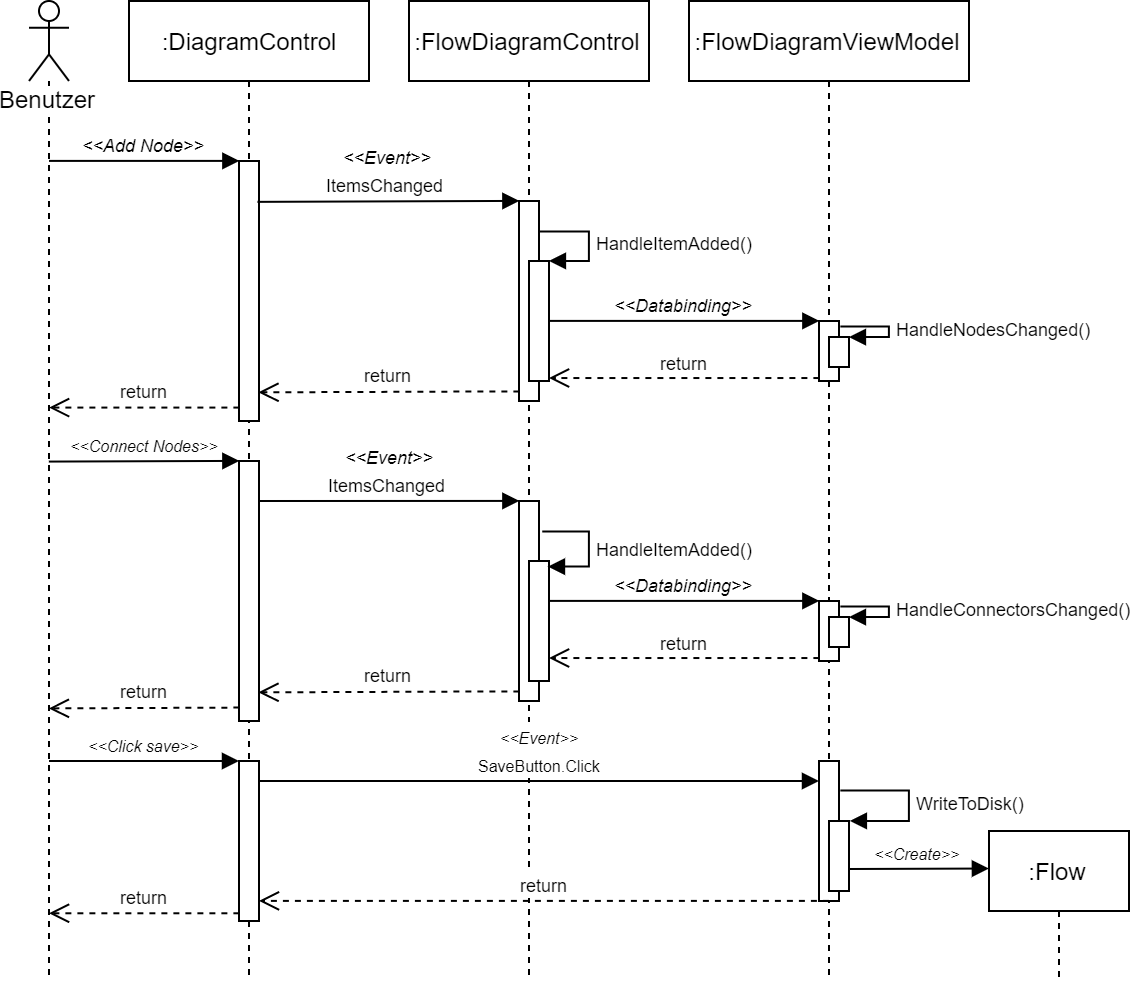
\includegraphics[width=\textwidth]{img/MVVMSequence.png}
	\caption[Kommunikationsablauf zwischen View- und ViewModel-Schicht]{Der Ablauf der Kommunikation zwischen der View- und der ViewModel-Schicht. Interagiert der Benutzer mit dem View, zum Beispiel durch das Hinzufügen von Nodes oder Connectors, werden entsprechende Events ausgelöst. Auf diese reagiert die abgeleitete View-Klasse FlowDiagramControl und aktualisiert ihre Daten mit den Objekten. Das ViewModel erhält die aktualisierten Daten über die Datenbindung des Frameworks und kann so, wenn der Benutzer das Konversationsrouting speichern möchte, die Klasse Flow der Model-Schicht instanzieren.}
	\label{fig:UML:MVVMSequence}
\end{figure}

\subsection[Die View-Schicht]{Die View-Schicht: FlowDiagramView, FlowDiagramControl, FlowDiagramItem}
Die View-Schicht übernimmt alle Elemente der grafischen Benutzeroberfläche, die der Benutzer unmittelbar sieht und mit denen er interagiert. Das Hauptelement der View-Schicht ist die Klasse FlowDiagramView, welche von der Framework-Klasse UserControl erbt. FlowDiagramView umfasst alle Windows Forms-Controls, die zum Darstellen des Editors benötigt werden und übernimmt zusätzlich die Konfiguration des MVVM-Frameworks während der Initialisierungsphase der Benutzeroberfläche.
\newline  
Das wichtigste Element der Benutzeroberfläche ist das Control FlowDiagramControl, welches  die abstrakte Syntax des Konversationsroutings darstellt. In Abbildung \ref{fig:UML:FlowView} ist schematisch dargestellt, wie es in die Klassenstruktur der View-Schicht eingefügt ist. Es basiert auf der Devexpress-Klasse DiagramControl, die es Benutzern ermöglicht, Diagramme mit geometrischen Formen und Verbindungen zu gestalten. FlowDiagramControl ist von dieser Klasse abgeleitet und erweitert sie um die Fähigkeit, ein Modell der DSL per Datenbindung darzustellen. Dafür sind in FlowDiagramControl Listen vom Typ ObservableCollection als Membervariablen angelegt, welche die Elemente des aktuellen DSL-Modells enthalten. Diese Listen existieren analog zur Klasse FlowDiagramViewModel aus Abschnitt \ref{subsec:Die Viewmodel-Schicht}. Durch die Datenbindung zwischen FlowDiagramControl und FlowDiagramViewModel werden die Inhalte aller Listen synchron gehalten. Die Aufgabe von FlowDiagramControl ist es, auf Interaktionen des Benutzers so zu reagieren, dass die Listen entsprechend aktualisiert werden. Zu diesem Zweck ist diese Klasse in einigen Aspekten gegenüber DiagramControl wie folgt angepasst und spezialisiert.
\newline
Für ein Devexpress-DiagramControl kann eine Auswahl von sogenannten Stencils, also für das Diagramm verfügbare Formen, dem Control hinzugefügt werden. Jedes Stencil verfügt über ein Objekt der Klasse FactoryItemTool, welches eine Instanz vom Interface-Typ IDiagramItem erzeugt. Wird ein Stencil aus der Toolbox in das Diagramm per Drag and Drop eingefügt, erzeugt das zugehörige FactoryItemTool ein entsprechendes Objekt, welches IDiagramItem implementiert. IDiagramItem stellt Methoden zu Verfügung, die DiagramControl benötigt um Objekte grafisch darzustellen. FlowDiagramControl ist so konfiguriert, dass jeder Node-Subtyp, also jede Instruktion der DSL, als eigenes Stencil dem Control hinzugefügt ist. Die Instanzen von FactoryItemTool für jedes dieser Stencil erzeugen ein Objekt vom Typ FlowDiagramItem. FlowDiagramItem ist die visuelle Repräsentation einer Konversationsrouting-Instruktion und erbt von der Devexpress-Klasse DiagramContainer, welche IDiagramItem implementiert. FlowDiagramItem besitzt eine Referenz auf ein Objekt vom Typ Node. Im Konstruktor von FlowDiagramItem wird das visuelle Erscheinungsbild einer einzelnen Instruktion initialisiert: Dabei werden Klassen vom Devexpress-Typ DiagramShape zu einer Liste hinzugefügt, welche dann vom Framework gezeichnet werden und verschiedene geometrische Formen annehmen können. FlowDiagramItem fügt der Liste von DiagramShapes ein blaues Rechteck für den Körper, ein weißes Rechteck für die Instruktionsüberschrift sowie kleinere rote und grüne Rechtecke für Instruktionsaus- und Eingänge hinzu. Die Rechtecke für Ein- und Ausgänge werden durch die eigens implementierten Klassen FlowDiagramInputPort und FlowDiagramOutputPort repräsentiert. Beide Klassen erben von der gemeinsamen Basis-Klasse FlowDiagramPort, welche wiederum DiagramContainer erweitert. Diese Port-Klassen bestimmen das visuelle Erscheinungsbild der zu zeichnenden Rechtecke und ermöglichen es FlowDiagramItem, Ausgänge zu beschriften oder aus- und einzublenden. Wieviele Aus- und Eingänge die jeweilige zu visualisierende Instruktion besitzt, wird aus dem Subtyp der Node-Referenz ermittelt, die in FlowDiagramItem hinterlegt ist.
\newline
Wird nun vom Benutzer ein Stencil aus der Toolbox ausgewählt und in das Modellierungsfenster gezogen, erzeugt die zugehörige Instanz von FactoryItemTool ein FlowDiagramItem. Dieses FlowDiagramItem wird mit einer Referenz auf eine neu erstellte Instanz des Node-Subtyps der ausgewählten Instruktion initialisiert. DiagramControl löst dann ein Event aus, das signalisiert, dass sich die Liste an Diagramm-Elementen verändert hat. FlowDiagramControl reagiert auf dieses Event seiner Basisklasse, indem es die Node-Referenz aus dem hinzugefügten FlowDiagramItem zu der Liste der Nodes hinzufügt, die per Datenbindung an das FlowDiagramViewModel gebunden sind. Umgekehrt reagiert FlowDiagramControl auch auf Events, die ausgelöst werden, wenn die Liste der Nodes durch das ViewModel verändert wird. In diesem Fall wird ein neues FlowDiagramItem mit einer Referenz auf die hinzugefügte Node erzeugt, sodass diese Node auf der Benutzeroberfläche zu sehen ist. Analog verhält sich das System wenn Nodes oder FlowDiagramItems gelöscht werden, nur dass in diesem Fall Elemente entfernt werden.
\newline
Um die Verbindungen zwischen Instruktionen zu modellieren, wird ähnlich vorgegangen. FlowDiagramControl überschreibt die geerbte Methode CreateConnector, welche vom Framework aufgerufen wird, wenn der Benutzer eine Verbindung zwischen Diagrammelementen zieht. Die Methode liefert eine Instanz von FlowDiagramConnector zurück, in der eine Referenz auf einen Connector der Model-Schicht hinterlegt ist. Wird ein FlowDiagramConnector dem Diagramm hinzugefügt, wird über ein entsprechendes Event ein neuer Connector der per Datenbindung synchronisierten Liste hinzugefügt. In FlowDiagramViewModel wird dementsprechend ebenfalls ein neuer Connector hinzugefügt und die Input- und Output-Referenzen der im Connector betroffenen Ein- und Ausgänge werden aktualisiert. Wird ein Connector der Modelschicht hinzugefügt, läuft der Prozess rückwärts ab. Das heißt, über die synchronisierte Liste der Connector-Instanzen wird ebenfalls im FlowDiagramControl ein Event ausgelöst, so dass das Control dem Diagramm einen neuen FlowDiagramConnector hinzufügen kann. Beim Entfernen von Connector-Instanzen wird der Prozess gleich behandelt, nur dass Referenzen entsprechend entfernt werden.      

\begin{figure} %[hbtp]
	\centering
		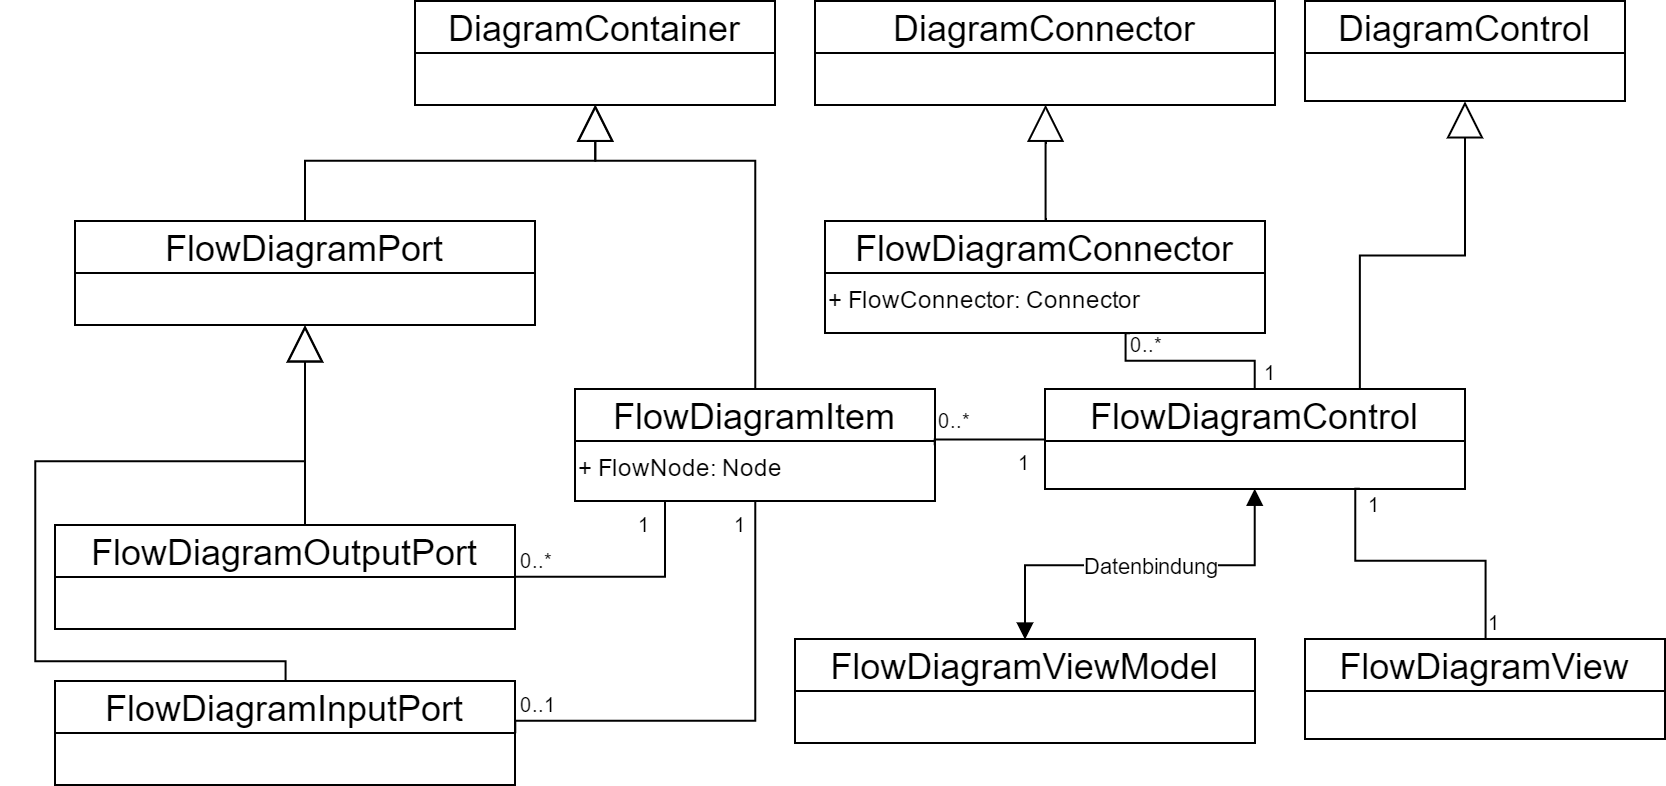
\includegraphics[width=\textwidth]{img/FlowViewUML.png}
	\caption[Klassenstruktur der View-Schicht]{Abgebildet ist ein Teil der View-Schicht. Zu sehen ist FlowDiagramView, welche über eine Instanz von FlowDiagramControl verfügt. FlowDiagramControl beinhaltet die Klassen FlowDiagramItem und FlowDiagramConnector, welche die Node- und Connector-Instanzen der Model-Schicht visualisieren. Über das ViewModel erhält FlowDiagramControl per Datenbindung Zugriff die zu visualisierenden Daten.}
	\label{fig:UML:FlowView}
\end{figure}


\section{Transformation}
\label{sec:Transformation}

\subsection{Konzept}
Die Transformation ist der Schritt in der Verarbeitungskette, in der aus einem semantischen Modell, welches in der Form der C\#-Datenstruktur aus Abschnitt \ref{subsec:Die Model-Schicht} vorliegt, die MSIL-Syntax generiert wird. Diese kann anschließend kompiliert und ausgeführt werden. Ein Modell wird auf eine zu generierende Klasse abgebildet, welche das gewünschte Verhalten des Modells implementiert. Diese Klasse erbt von einer abstrakten Basisklasse mit dem Namen ACDCallRoutingBehaviorBase, welche die abstrakte Methode StartAsync zur Verfügung stellt. Die vom Transformationsalgorithmus generierte Klasse implementiert StartAsync so, dass beim Aufruf das vom Benutzer spezifizierte Konversationsrouting abgespielt wird.
\newline 
Die Instruktionen des Konversationsroutings werden als Membermethoden der Klasse abgebildet. In der generierten Klasse existiert für jede Instruktion eine eigene Methode, deren Syntax das gewünschte Verhalten der Instruktion umsetzt. Der Bezeichner der Methode trägt den Namen der Instruktion, gefolgt von einer eindeutigen Identifikationsnummer, sodass mehrere Instruktionen des gleichen Typs bei der Generierung der zugehörigen Membermethoden nicht kollidieren. Manche Instruktionen müssen mit der zu routenden Konversation interagieren. Zu diesem Zweck steht der generierten Klasse eine API zur Verfügung, welche aus einer Instanz eines Interfaces namens IRoutedAcdCall besteht. Soll beispielsweise im Zuge einer Media Playback-Instruktion eine Audio-Datei abgespielt werden, kann Syntax generiert werden, welche die Methode PlayAudioAsync des Interfaces IRoutedAcdCall aufruft. 
\newline
Die Reihenfolge von Instruktionen in einem Konversationsrouting wird realisiert, indem generierte Methoden die Methoden ihrer Nachfolgeinstruktionen aufrufen. Angenommen, eine Branch-Instruktionen hat zwei Ausgänge: Der ''True``-Ausgang zeigt auf eine Media Playback-Instruktion während der ''False``-Ausgang auf die Terminate-Instruktion verweist. Aus diesen drei Instruktionen wird Syntax für drei Membermethoden generiert: Die Methode der Branch-Anweisung wertet den per Parameter übergebenen booleschen Ausdruck aus und ruft im True-Fall die Methode der Media Playback-Instruktion auf. Andernfalls wird die Methode der Terminate-Anweisung aufgerufen. Da es sich bei dem semantischen Modell um einen Graphen und keinen Baum handelt, kann es in Modellen zu Zyklen kommen. Solche potentiell endlose Konversationsroutings stellen ein Problem dar, denn sie führen zu einer endlosen Rekursion von Methodenaufrufen innerhalb der generierten Klasse. Das Problem wird gelöst indem eine Instruktion, die eine solche Rekursion starten würde, die nächste Instruktion in einem .NET-Task auf einem neuen Thread aufruft. Der aktuelle  Thread terminiert an der Stelle, an der der neue gestartet wird und eine endlose Rekursion wird vermieden.
\newline
Ein Modell kann vom Benutzer geschriebenen C\#-Code enthalten. Dieser muss in die generierte Klasse integriert werden, um ausführbar zu sein. Benutzerdefinierten Code jedoch einfach in die Syntax für Membermethoden einzufügen birgt Risiken. So hätte der Benutzer in seinem selbstgeschriebenen Code Zugriff auf alle Elemente der generierten Klasse, was zu Problemen führen kann, wenn er Methoden aufruft, die der generierten Klasse vorbehalten sind. Stattdessen wird Code des Benutzers wird in einer verschachtelten privaten Klasse gekapselt. Die geschachtelte Klasse trägt den Bezeichner ``UserCode'' und kapselt den benutzerdefinierten Code in eigenen Membermethoden. Die umfassende Klasse verfügt als Membervariable eine Instanz der Klasse UserCode und kann so den Code des Benutzers ausführen. Ist beispielsweise eine Script-Instruktion im Konversationsrouting integriert, wird der Skript-Code als eigene Membermethode in der Klasse UserCode angelegt. Die Skript-Instruktion wird zusätzlich als Membermethode der umfassenden Klasse abgebildet, welche dann die zugehörige Membermethode der Klasse UserCode aufruft. Da Scripte einen String zurückliefern (siehe \ref{subsec:Script}), gibt auch die in UserCode angelegte Membermethode einen String zurück, welcher dann in der aufrufenden Methode verwertet wird.
\newline
Vom Benutzer definierte Variablen und Funktionen sind in allen Instruktionen verwendbar, in denen der Benutzer eigenen Code angeben kann. Da Code des Benutzers in der Klasse UserCode abgebildet wird, werden auch die vom Benutzer angelegten Variablen und Funktionen in dieser Klasse jeweils als private Membervariablen und -funktionen angelegt. Die vordefinierten Variablen Skill und Language sind ebenfalls über die Klasse UserCode verfügbar: Sie sind als Properties von UserCode implementiert, die beim Benutzen per Getter und Setter über eine Instanz eines Interfaces namens IPredefinedVariables gesetzt werden. In der Routing Engine werden für Sprachen und Wissensbereiche interne Datenstrukturen verwendet. PredefinedVariable bildet die im System verfügbaren Sprachen und Wissensbereiche auf leicht handhabbare Strings ab, damit der Benutzer in seinen Skripten nicht mit ganzen Datenstrukturen arbeiten muss. Er setzt lediglich den String der gewünschten Variable und die Implementierung von IPredefinedVariable sucht die Datenstruktur mit dem gleichen Namen und setzt die entsprechende Variable.
\newline
Einige Aufrufe der API zur Interaktion mit dem eingehenden Ruf müssen den Programmfluss des Konversationsroutings zeitweise blockieren. So muss beispielsweise bei der Ausführung einer Media Playback-Instruktion darauf gewartet werden bis die Audiodatei zu Ende ist, bevor das Konversationsrouting weiter ausgeführt werden kann. In der Umsetzung wird zu diesem Zweck .NETs System der asynchronen Methodenausführung genutzt, welches den aktiven Thread der Routing Engine nicht blockiert (siehe \ref{subsec:Asynchrone Methodenausfuehrung}). Dazu werden Instruktionen, welche blockierende oder asynchrone API-Methoden aufrufen, selber auf asynchrone Methoden abgebildet. Die API-Methoden werden dann mithilfe des ``await''-Operators aufgerufen. Dies hat zur Folge, dass alle Methoden, die asynchrone Methoden im Zuge des Konversationsroutingablaufs aufrufen, diese ebenfalls mit ``await'' aufrufen und daher selber zu asynchronen Methoden werden. Folgt einer Set Variables-Instruktion beispielsweise eine Media Playback-Instruktion, so wird die Media Playback abbildende Methode mit einem await aufgerufen, während die Set Variable abbildende Methode selber als ``async'' deklariert wird. Der Aufrufer von Set Variables muss anschließend selber async werden, und so weiter. Dieses Muster zieht sich durch bis zu StartAsync-Methode, welche der Einstiegspunkt jedes Konversationsroutings ist.

\subsection{Beispiel}
\label{subsec:Beispiel}
Folgendes Beispiel soll die Transformation eines Konversationsroutings zu CIL-Syntax besser veranschaulichen. In Abb. \ref{fig:FlowToCode} ist ein einfaches Konversationsrouting dargestellt. 

\begin{figure} %[hbtp]
	\centering
		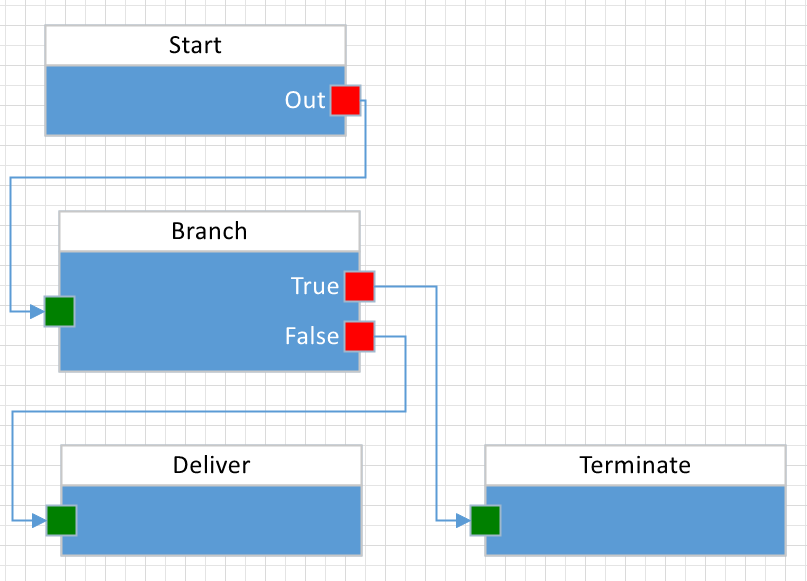
\includegraphics[width=0.7\textwidth]{img/FlowToCodeExample.png}
	\caption[Beispielhaftes Konversationsrouting zur Veranschaulichung der Transformation zu C\#-Syntax]{Beispielhaftes Konversationsrouting zur Veranschaulichung der Transformation zu CIL-Syntax.}
	\label{fig:FlowToCode}
\end{figure}

Die CIL-Syntax, die aus einem solchen Modell generiert wird, sieht in C\# dargestellt folgendermaßen aus:
\newpage

\lstinputlisting[breaklines=true, style=sharpc]{code/FlowToCode.cs}

Bei diesem Beispiel ist zu beachten, dass bei der Transformation nicht wirklich konkrete C\#-Syntax generiert wird, sondern ihr abstraktes Gegenstück in Form eines Rosyln-SyntaxTree-Objekts. Für die Illustration des Transformationskonzeptes ist die Syntax hier jedoch konkret dargestellt.
\newline
Am Anfang des Listings steht die Deklaration einer öffentlichen Klasse namens GeneratedConversationBehavior, die von ACDCallRoutingBehavior erbt. Dies ist die Klasse, in der die Instruktionen als Membermethoden abgebildet werden. In dieser Klasse wird als nächstes eine private Klasse UserCode definiert. In UserCode sind die vordefinierten Variablen Skill und Language definiert, welche über ihre Getter und Setter auf eine private Instanz des Interfaces IPredefinedVariable zugreifen. Zusätzlich existiert eine Methode mit dem Namen ''BranchNode'' gefolgt von einer einzigartigen Kennnummer. Diese Methode enthält den vom Benutzer spezifizierten Ausdruck der für die Branch-Instruktion ausgeführt werden soll. Dementsprechend wird ein boolescher Wert zurückgeliefert. In diesem Beispiel vergleicht die Branch-Instruktion also die aktuelle Sprache, welche in der vordefinierten Variable Language gespeichert ist, mit dem String ``Deutsch''. 
\newline
Nach der Klasse UserCode folgt die eigentliche Implementierung des Konversationsroutings. Im Konstruktor der Klasse GeneratedConversationBehavior werden Abhängigkeiten zum Rest des Systems initialisiert: So wird mittels einer Instanz des Interfaces IRoutedAcdCall auf eine API zur Beeinflussung des eingehenden Anrufes zugegriffen. Die beiden Instanzen von IReadOnlyRepository stellen Methoden zur Verfügung, um auf die dem System bekannten Sprachen und Wissensbereiche zuzugreifen. Die drei Interface-Instanzen werden an die Basisklasse ACDCallRoutingBehaviorBase weitergeleitet. Im Konstruktor wird außerdem die private Instanz von UserCode initialisiert, welcher eine Instanz des PredefinedVariables-Interface aus der Basis-Klasse übergeben wird. Die restlichen Methoden der Klassen stellen die Abbildung der Instruktionen des Konversationsroutings dar. Die Start-Instruktion wird auf die Methode ``StartAsync'' abgebildet. Hier wird dem Routing gemäß sofort die Methode der Branch-Instruktion ``BranchNode'' aufgerufen, welche zuerst den vom benutzerdefinierten Code aus der Klasse UserCode aufruft, und das Ergebnis dessen als Bedingung in eine If-Abfrage einsetzt. Je nachdem welches Ergebnis zurückgeliefert wird, wird entweder die Methode der Deliver- oder der Terminate-Instruktion aufgerufen. ``TerminateNode'' ruft über die Membervariable Conversation der Basisklasse die API-Methode ``TerminateAsync'' auf, welche den eingehen Anruf beendet. Ähnlich läuft es in ``DeliverNode'' ab: Hier wird der Ruf mittels der API-Methode ``DeliverAsync'' der Ruf an einen Agenten zugestellt. Die dabei übergebene SIP-URI ist ein Parameter der Deliver-Instruktion.
\newline
Wird die Klasse GeneratedConversationBehavior nun von der RoutingEngine instanziert, und in einer Variable vom Typ ACDCallRoutingBehaviorBase gespeichert, kann über die Methode ``StartAsync'' das vom Benutzer gewünschte Konversationsrouting abgespielt werden.

\subsection{Umsetzung}
Das oben beschriebene Konzept zur Abbildung des semantischen Modells auf MSIL-Syntax wird von einer eigenen API realisiert, welche von der Routing Engine benutzt wird. Die grobe Klassenstruktur dieser API ist in Abbildung \ref{fig:UML:Transformator} zu sehen. Das Hauptelement ist die Klasse ConversationRoutingBehaviorGenerator, welche das Interface IBehaviorGenerator implementiert. Dieses Interface stellt die Methode GenerateAssembly zur Verfügung, welche ein semantisches Modell in Form einer Flow-Instanz entgegennimmt und eine MSIL-Assembly zurückliefert.  Dafür muss das semantische Modell jedoch zuerst in einen CIL-Syntaxbaum konvertiert werden. Zum Erstellen des Syntaxbaums wird die Methode BuildTree des Interfaces ISyntaxTreeBuilder verwendet, welches von der Klasse ConversationRoutingSyntaxTreeBuilder implementiert wird. BuildTree nimmt den Start-Knoten des Konversationsroutings sowie die benutzerdefinierten Variablen und Funktionen entgegen, und liefert einen kompilierbaren Syntaxbaum zurück. Der Syntaxbaum wird aus kleineren Einheiten zusammengesetzt: Auf der höchsten Ebene stehen die Klassendeklarationen, welche wiederum die Membermethodendeklarationen beinhalten. Wie diese Einheiten generiert werden, wird in den folgenden Abschnitten erläutert.

\begin{figure} %[hbtp]
	\centering
		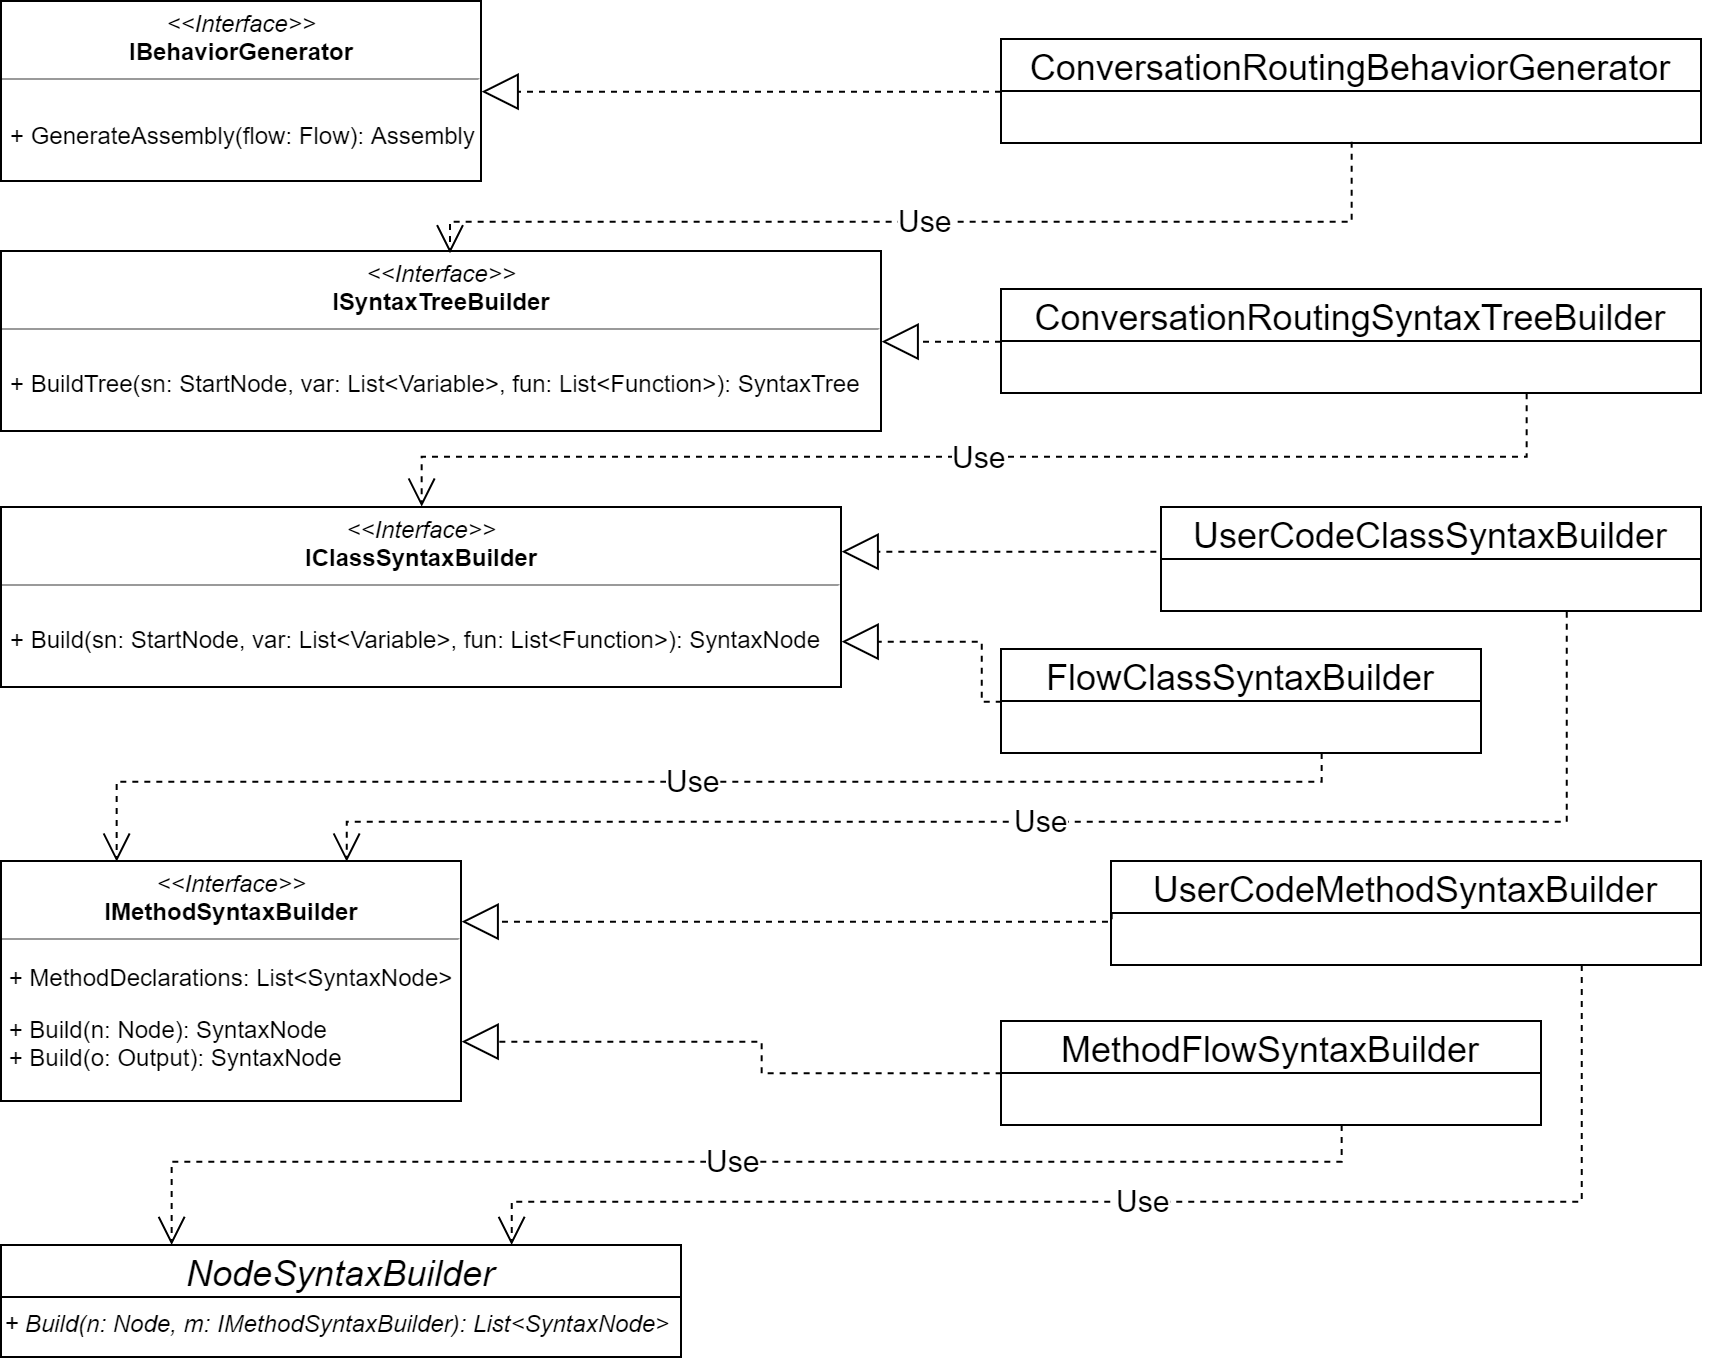
\includegraphics[width=\textwidth]{img/TransformatorUML.png}
	\caption[Klassenstruktur des Transformators]{Zu sehen ist die Klassenstruktur des Transformators. Die Hauptfunktionalitäten sind in den Interfaces abgebildet. Für die Implementierung dieser Methoden sind wiederum Funktionalitäten notwendig, die in anderen Interfaces definiert sind.}
	\label{fig:UML:Transformator}
\end{figure}
 

\subsubsection{Programmablauf}
\label{subsubsec:Programablauf}
Die Grundidee der Syntax-Zusammensetzung orientiert sich an einem Verfahren, das in \cite[S. 272f]{Voelter:13} als ''klassische Modell-Transformierung`` (engl. classical model transformation) bezeichnet wird: Das semantische Modell wird als Graph traversiert, während mit der Roslyn-API anhand des aktuell besuchten Knotens die passende Syntax generiert wird. Die Traversierung beginnt bei dem Start-Knoten des Konversationsroutings und besucht jede Instruktion des Graphen in der Reihenfolge einer Tiefensuche. Pro besuchter Instruktion wird die CLI-Syntax für eine Methode erstellt, welche das Verhalten der Instruktion umsetzt. Dort wo die Syntax die Methode der nachfolgenden Instruktion aufruft, wird diese Instruktion rekursiv besucht und die entsprechende Syntax für die abbildende Methode erstellt. Dies geht so lange weiter, bis eine Instruktion erreicht wird, die keine ausgehenden Verbindungen hat. An dieser Stelle ist der Rekursionsanker erreicht: Die Syntax für die letzte Instruktion des aktuellen Pfades wird generiert, der Liste der Membermethoden hinzugefügt, und der Aufruf der so generierten Methode an die Vorgänger-Instruktion zurückgeliefert. Diese kann den erhaltenen Aufruf nun in ihre eigene Syntax integrieren und ihren eigenen Aufruf an die eigene Vorgänger-Instruktion zurückliefern. Der Programmfluss kehrt auf diese Weise zurück zur Start-Instruktion, wo der letzte Methodenaufruf in die Methode ``StartAsync'' integriert wird. Zu diesem Zeitpunkt sind alle Methodendeklarationen erstellt und können der Klassendeklaration hinzugefügt werden. 
\newline
Da es sich bei einem Konversationsrouting auch um einen zyklischen Graph handeln kann, muss überprüft werden, ob ein solcher Zyklus im Routing vorhanden ist, um eine endlose Rekursion zu vermeiden. Daher wird während des rekursiven Ablaufs mit einem Stapelspeicher Protokoll geführt, welche Knoten des Routings schon besucht wurden. Beim Besuchen eines Knotens wird dieser auf den Stapel gelegt, beim Verlassen auf dem Rückweg der Rekursion wird dieser wieder entnommen. Wird ein Knoten besucht, der sich schon auf dem Stapelspeicher befindet, ist dieser Teil eines Zyklus und die Rekursion kann abgebrochen werden. Der zurückzuliefernde Methoden-Aufruf für diesen Knoten wird dann in einem neuen Thread ausgeführt. 
\newline
Die Struktur der Klassen, die den obenstehenden Algorithmus umsetzen, ist in Abbildung \ref{fig:UML:Transformator} zu sehen. Die Klasse FlowClassSyntaxBuilder implementiert die Schnittstelle IClassSyntaxBuilder, welche die Methode Build zur Verfügung stellt. Build nimmt eine Referenz auf die StartNode entgegen und liefert eine Klassendeklaration in Form einer SyntaxNode zurück. SyntaxNode ist ein Typ der Roslyn-API, welcher einen Knoten im CIL-Syntaxbaum repräsentiert. FlowClassSyntaxBuilder implementiert IFlowClassSyntaxBuilder indem es die Syntax für die zu generierende Klasse erstellt. Zum Erstellen der Membermethoden der Klasse wird das Interface IMethodSyntaxBuilder benutzt, welches von der Klasse MethodFlowSyntaxBuilder implementiert wird. IMethodSyntaxBuilder stellt Methoden zur Verfügung, welche Instanzen von Node oder Output entgegennehmen und eine Methodendeklaration zurückliefern, welche die übergebene Node abbilden soll. MethodFlowSyntaxBuilder implementiert diese Methoden mithilfe des rekursiven Prozesses, der weiter oben erläutert ist. Zu diesem Zweck implementiert die Klasse das Visitor-Pattern in Form des Interfaces IFlowNodeVisitor, in dem Methoden bereit gestellt werden, mit der alle Node-Subtypen sowie Inputs und Outputs besucht werden können (vgl. \cite[S. 5f]{Jones}, wo dieses Verfahren für abstrakte Syntaxbäume empfohlen wird). Bei dem Besuch einer Node muss je nach Subtyp bestimmte konkrete CIL-Syntax erstellt werden. Zu diesem Zweck existiert die abstrakte Klasse NodeSyntaxBuilder, von der pro Node-Subtyp eine Klasse erbt. Jeder dieser erbenden Klassen generiert die Syntax für den jeweiligen Node-Subtyp, für den sie zuständig ist. Dies geschieht in der überschriebenen Build-Methode der Basisklasse NodeSyntaxBuilder, welche die Syntax an MethodeFlowSyntaxBuilder zurückliefert. Der Ablauf ist in den Diagrammen \ref{fig:UML:TransformationSequence} und \ref{fig:UML:TransformationSequenceDetail} abgebildet und wird wie folgt abgewickelt:
\newline
Zuerst wird die Build-Methode für die StartNode-Referenz eines Flows aufgerufen, in der eine Instanz von StartNodeSyntaxBuilder erzeugt wird. Auf dieser Instanz wird nun die Methode Build aufgerufen, welcher neben der Referenz auf die StartNode auch die aufrufende Instanz von MethodFlowSyntaxBuilder übergeben wird. So kann StartNodeSyntaxBuilder für die Output-Instanz des StartKnotens MethodFlowSyntaxBuilder.Build aufrufen, in der wiederum die Visit-Methode aufgerufen wird. In der Visit-Methode wird nun Visit für die Input-Instanz aufgerufen, auf die der Output der StartNode verweist. Dort wird erneut Visit für die Node-Instanz aufgerufen, auf die wiederum der Input verweist. Die Rekursion setzt sich hier fort: Es wird ein NodeSyntaxBuilder für die aktuell besuchte Node instanziert und Build aufgerufen. Innerhalb der Build-Methode des NodeSyntaxBuilders wird jetzt die CIL-Syntax für die Instruktion in Form einer Liste von SyntaxNodes erstellt. Hat die aktuelle Node weitere Output-Instanzen, wird auch hier wieder MethodFlowSyntaxBuilder.Build für diese aufgerufen. Handelt es sich jedoch um eine Instruktion ohne Ausgänge, ist der Rekursionsanker erreicht. Der aktuelle NodeSyntaxBuilder liefert seine Liste mit SyntaxNodes an den MethodFlowSyntaxBuilder.Visit-Aufruf zurück. Dort werden die SyntaxNodes zu einer Methodendeklaration zusammengefasst und gespeichert. Der Visit-Aufruf kehrt zu seinem Build-Aufruf zurück und gibt als Rückgabe-Wert eine SyntaxNode zurück, in der ein Aufruf der eben erstellten Methodendeklaration enthalten ist. Dieser Aufruf kehrt zu dem Build-Aufruf des StartNodeSyntaxBuilder zurück, der die Syntax der StartNode generiert. Dort kann der Aufruf nun in die Syntax der eigenen Methode integriert werden, welche ihrerseits nun zu MethodFlowSyntaxBuilder zurückkehrt und der StartNode-Methode hinzugefügt wird. Der Prozess wird für alle Instruktionen eines Konversationsroutings durchgeführt, sodass am Ende die Programmfluss-Struktur aus Abschnitt \ref{subsec:Beispiel} erreicht ist.

\begin{figure} %[hbtp]
	\centering
		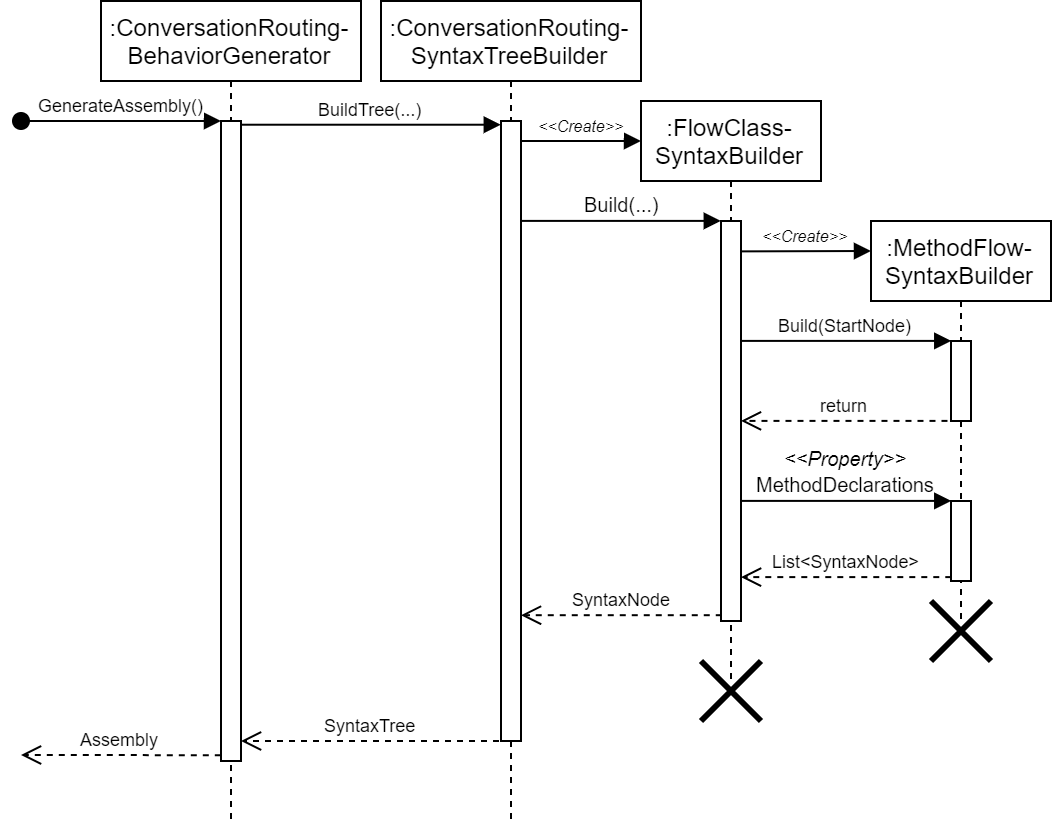
\includegraphics[width=\textwidth]{img/TransformationSequence.png}
	\caption[Transformatinosablauf]{Grober Ablauf der Transformation als Sequenzdiagramm. Für den detailierten Ablauf in MethodFlowSyntaxBuilder siehe Abb. \ref{fig:UML:TransformationSequenceDetail} }
	\label{fig:UML:TransformationSequence}
\end{figure}

\begin{figure} %[hbtp]
	\centering
		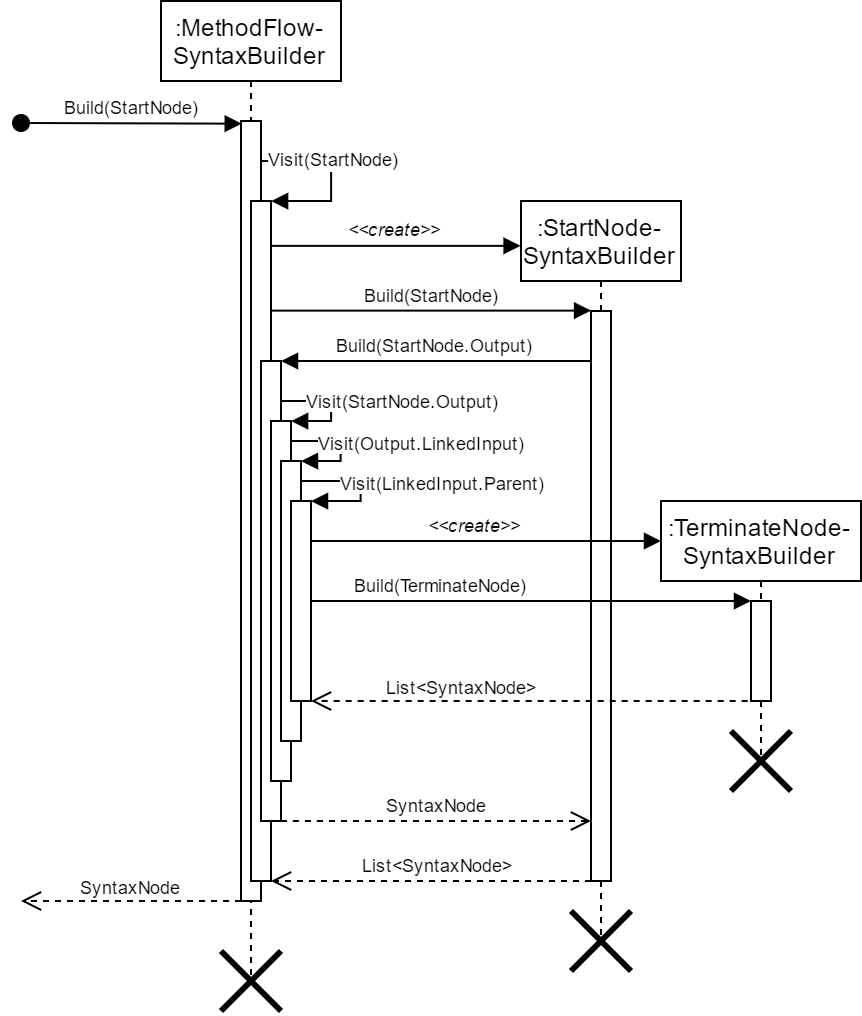
\includegraphics[width=0.8\textwidth]{img/TransformationSequenceDetail.png}
	\caption[Transformationsablauf im Detail]{Ablauf der Generierung der Methodensyntax im Detail. Zu sehen ist der rekursive Ablauf des Verhaltens der Klasse MethodFlowSyntaxBuilder. In dem abgebildeten Diagramm ist der Ablauf zur Erstellung einer Syntax für ein Konversationsrouting  abgebildet, bei dem die Start-Instruktion direkt in die Terminate-Instruktion mündet. Das Beispiel ist so simpel gehalten um die Komplexität des Diagramms nicht unnötig zu erhöhen.}
	\label{fig:UML:TransformationSequenceDetail}
\end{figure}

\subsubsection{Nebenläufigkeit}
\label{subsubsec:Nebenlaeufigkeit}
Wie in Abschnitt \ref{sec:Transformation} beschrieben, werden manche Instruktionen auf asynchrone Methoden abgebildet, deren Asynchronität sich durch ein Konversationsrouting ziehen kann. Zum Zeitpunkt der oben beschriebenen Generierung der Programmablauf-Syntax muss bekannt sein, welche Instruktionen auf asynchrone Methoden abgebildet werden müssen. Daher wird vor der eigentlichen Generierung ein Vorverarbeitungsschritt ausgeführt, in dem alle Instruktionen des Konversationsroutings gesammelt werden, die auf asynchrone Methoden abgebildet werden müssen. Dafür wird das Konversationsrouting traversiert und asynchrone Instruktionen, sowie Instruktionen über die solche erreicht werden können, werden in einer Liste vermerkt, welche anschließend FlowClassSyntaxBuilder zur Verfügung gestellt wird. Die Bestimmung, ob eine Instruktion über einen Pfad im Routing eine asynchrone Instruktion erreichen kann, wird über die Berechnung der reflexiv-transitiven Hülle des Konversationsroutings, also einer Liste der direkten und indirekten Vorgänger aller Instruktionen, erreicht. So ist eine Instruktion asynchron, wenn sie in der reflexiv-transitiven Hülle in Relation mit einer anderen asynchronen Instruktion steht.

\subsubsection{Benutzerdefinierter Code}
Vom Benutzer spezifizierter Code wird in einer generierten Klasse namens UserCode gekapselt. Die Syntax für die Deklaration dieser Klasse wird von einer weiteren Implementierung des Interfaces IClassSyntaxBuilder namens UserCodeClassSyntaxBuilder übernommen. Da die UserCode-Klasse eine private Klasse ist, muss ihre Deklaration der Syntax für die Routing-steuernde Klasse hinzugefügt werden. Daher wird UserCodeClassSyntaxBuilder von FlowClassSyntaxBuilder benutzt. Die beiden Klassen ähneln sich in der Art und Weise, wie sie die Syntax für die jeweils eigene Klassendeklaration generieren: UserCodeClassSyntaxBuilder verwendet den gleichen rekursiven Ablauf zur Traversierung eines Konversationsroutings wie in Abschnitt \ref{subsubsec:Programablauf} beschrieben, nur dass dieser in seiner eigenen Klasse namens UserCodeMethodSyntaxBuilder implementiert ist. UserCodeMethodSyntaxBuilder behandelt beim Besuchen der Instruktionen nur Node-Subtypen, in denen benutzerspezifizierter Code zu finden ist. Für diese Knoten werden bestimmte NodeSyntaxBuilder-Subtypen instanziert, welche den Code des Benutzers parsen und in die zu erstellenden Methodendeklarationen der UserCode-Klasse einbetten. Außerdem bearbeitet UserCodeClassSyntaxBuilder auch die benutzerdefinierten Variablen und Funktionen. Diese werden der Reihe nach durchgegangen und die entsprechend generierte Syntax in Form von Methoden- und Variablendeklarationen wird der Klasse UserCode hinzugefügt. Die so entstehende UserCode-Klassendeklaration wird an FlowClassSyntaxBuilder übergeben, wo sie als private geschachtelte Klassendeklaration in die umfassende Klasse eingebettet wird.

\section{Modell-Validierung} 
Eine Aufgabe der DSL ist die Unterstützung des Benutzers, indem Fehler vermieden oder schnell beseitigt werden. Dafür ist es von hoher Bedeutung, dem Benutzer Fehlerzustände in einem Konversationsrouting frühzeitig anzuzeigen, damit diese nicht bei der weiteren Modellierung oder Transformation fortbestehen oder sich sogar vervielfachen. Zu diesem Zweck wird während der Modellierung im Editor eine Modell-Validierung durchgeführt, bei der sogenannte Constraints überprüft werden. Bei Constraints handelt es sich laut \cite[S. 82ff, 289ff]{Voelter:13} um Einschränkungen für die Gültigkeit eines DSL-Modells, welche dabei helfen, Fehler vor der endgültigen Transformation zu entdecken. Daher wird nach jeder Benutzer-Aktion, die das Konversationsrouting verändert, das aktuelle DSL-Modell analysiert und verschiedenen Prüfungen unterzogen. Diese Prüfungen stellen sicher, dass alle Constraints eingehalten werden und zeigen dem Benutzer im Falle eines Verstoßes eine entsprechende Fehlermeldung an.
\newline
Die Modell-Validierung findet im Editor statt. Dort steht dem ViewModel eine Instanz des Interfaces IFlowValidator zur Verfügung, dessen Klassenstruktur im Diagramm \ref{fig:UML:FlowValidatorClassStructure} abgebildet ist. Die Klasse FlowValidator implementiert IFlowValidator, welche die Methode Validate zur Verfügung stellt. Validate nimmt ein semantisches Modell in Form einer Flow-Instanz entgegen und liefert eine Liste von FlowDiagnostics zurück, in denen Details zu auftretenden Fehlern wie zum Beispiel eine Fehlernachricht oder die betroffene Instruktion gespeichert sind. Zur Implementierung des Interfaces benutzt FlowValidator eine Liste von Instanzen des Interfaces IConstraintEvaluator, welche die Methode Evaluate bereitstellt. Klassen, die IConstraintEvaluator implementieren, nehmen in der Evaluate-Methode einen Flow entgegen und überprüfen diesen auf einen einzelnen Constraint. Verletzt das semantische Modell diesen Constraint, liefert Evaluate eine Liste mit FlowDiagnostics zurück. In der vorliegenden Implementierung sind vier ConstraintEvaluators umgesetzt: 
\begin{description}
\item[StartNodeExistsEvaluator] \hfill \\
Dieser ConstraintEvaluator überprüft, ob im semantischen Modell eine einzelne Start-Instruktion vorhanden ist.
\item[NoUnconnectedNodeExistsEvaluator] \hfill \\
Hier wird überprüft, ob Instruktionen existieren, deren Eingang mit dem Rest des Konversationsroutings unverbunden ist. Für jede unverbundene Instruktion wird eine Instanz von FlowDiagnostic zurückgeliefert, in der die betreffenden Nodes referenziert sind.
\item[NodeParametersAreValidEvaluator] \hfill \\
NodeParametersAreValidEvaluator überprüft, ob die Parameter von allen Nodes zulässig sind. So dürfen zum Beispiel für Media Playback-Instruktion die angegebenen Audio-Dateien nicht null sein. Verstößt eine Node gegen Constraints dieser Art, wird sie in der zurückgelieferten Liste der FlowDiagnostics mit einer entsprechenden Warnung referenziert.
\item[UserCodeCompilesEvaluator] \hfill \\
UserCodeCompilesEvaluator prüft, ob der vom Benutzer geschriebene Code valide ist und kompiliert. Dafür muss das gesamte Modell transformiert und kompiliert werden. Daher besitzt UserCodeCompilesEvaluator eine Referenz auf eine ConversationRoutingBehaviorGenerator-Instanz, mit der bei jedem Aufruf von Evaluate das übergebene Modell transformiert wird. Statt einer Assembly wird von der Generator-Instanz allerdings das von Roslyn bereitgestellte semantische Modell der entstehenden CIL-Syntax angefordert. In diesem Objekt speichert die Rosyln-API unter anderem alle Diagnostiken zur generierten Syntax. Existieren solche Diagnostiken nach der Modell-Transformation, werden diese von der Evaluate Funktion in FlowDiagnostics umgewandelt und zurück geliefert.
\end{description}
Wird im FlowViewModel des Editors nun eine Aktion des Benutzers registriert, wird FlowValidator.Validate aufgerufen. Dort wird auf allen Instanzen von IConstraintEvaluator die Evaluate-Methode aufgerufen, die zurückgelieferten FlowDiagnostics gesammelt, und diese anschließend zurückgeliefert. In FlowViewModel werden die FlowDiagnostics nun in einer Liste gespeichert, die per Datenbindung an die View-Schicht gebunden ist. Die FlowDiagnostics werden in einer List-Control angezeigt, welche die Diagnostics in Form einer Fehlermeldung visualisiert und bei einem Mausklick auf die betroffene Instruktion verweist. Zwischen FlowDiagramViewModel und CodeEditorViewModel werden die FlowDiagnostics mit einem Nachrichten-Service ausgetauscht, der vom Devexpress-Framework angeboten wird. CodeEditorViewModel kann so die Diagnostiken in einer eigenen Liste anzeigen und die Fehler rausfiltern, die nicht den vom Benutzer geschriebenen Code betreffen. Zusätzlich können Fehler so im Code des Benutzers rot unterstrichen werden.

\begin{figure} %[hbtp]
	\centering
		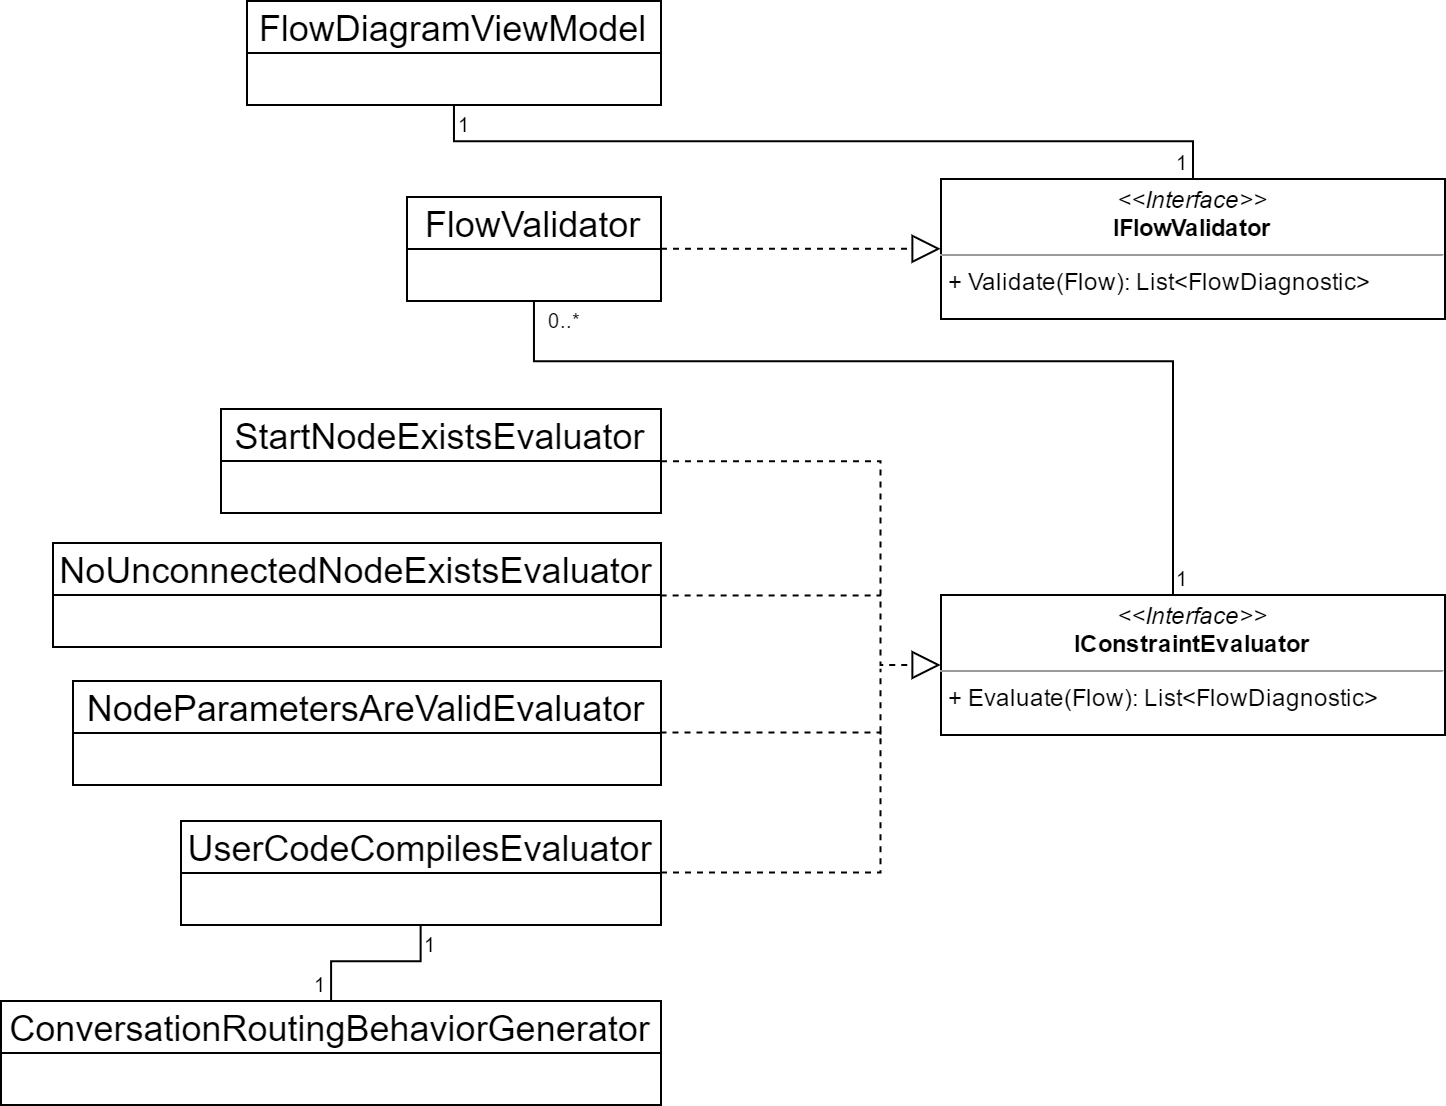
\includegraphics[width=\textwidth]{img/FlowValidatorClassStructure.png}
	\caption[Klassenstruktur der Modell-Validierung]{Abgebildet ist die Klassenstruktur der Modell-Validierung. Die Klasse FlowValidator benutzt eine Reihe von IConstraintEvaluator-Instanzen, um die etwaige Constraint-Verstöße eines Modells als eine Liste von FlowDiagnostics an das ViewModel weiterzuleiten.}
	\label{fig:UML:FlowValidatorClassStructure}
\end{figure}
\chapter{Evaluierung}

\section{Test}
Die Verifikation der DSL und ihrer Komponenten wird auf zwei Arten durchgeführt: Zum einen mit automatisierten Modultests und zum anderen mit manuellen Integrationstests. Erstere zielen darauf ab die Funktionsweise von Editor, Transformator und Validierer einzeln zu testen, um zu verifizieren dass diese ihre Anforderungen erfüllen. Letztere sollen das Zusammenspiel aller Module der DSL prüfen indem der Erstellungsprozess für verschiedene Konversationsroutings von der Modellierung bis zur Ausführung des Routings nachvollzogen wird.

\subsection{Automatisierte Tests}
Für die automatisierten Tests der DSL-Komponenten kommen Modultests, auch Unit Tests genannt, zum Einstaz. Befürworter der Unit Testing-Praktik befürworten an dieser Technik unter anderem eine hohe Testabdeckung und die frühe Detektierung von Fehlerzuständen [CITATION]. In der vorliegenden Ausarbeitung wird das Unit Test-Verfahren mit Hilfe des .NET-Test-Frameworks XUnit umgesetzt. Dabei werden Methoden mit einem Attribut als Test-Methoden designiert, welche dann von XUnit ausgeführt und ausgewertet werden. Die Testmethoden folgen dem Arrange-Act-Assert-Entwicklungsmuster. Hierbei ist eine Methode in drei Phasen aufgeteilt: In der Arrange-Phase werden die für den Test nötigen Vorbereitungen wir Objekt-Initialisierungen etc. durchgeführt. Anschließend folgt die Act-Phase, in der die zu testende Aktion durchgeführt wird. In der Assert-Phase wird das Testergebnis mit Assertions überprüft. Schlägt keine der Assertions fehl, gilt ein Testfall als bestanden.

\subsubsection{Editor}
In der Editor-Komponente werden zwei Klassen getestet: FlowDiagramViewModel und FlowDiagramControl. Die beiden Komponenten sind vor allem über die Datenbindung des Devexpress-Frameworks miteinander verbunden. Da das Testen dieser Verbindung jedoch außerhalb des Zuständigkeitsbereichs für die vorliegende Ausarbeitung ist, werden die beiden Klassen unabhängig voneinander getestet. Für FlowDiagramViewModel ist besonders das Verhalten bei Veränderungen in der Model-Schicht interessant, vor allem wenn es um das Hinzufügen oder Entfernen von Verbindungen geht. Folgende Aspekte der Klasse FlowDiagramViewModel werden unter anderem in den vorliegenden Unit Tests verfiziert: 

\begin{itemize}
\item Das Speichern von Flow-Instanzen im Dateisystem funktioniert
\item Das Laden von Flow-Instanzen aus dem Dateisystem funktioniert
\item Beim Hinzufügen von Connector-Instanzen werden die zugehörigen Input-Referenzen in betroffenen Outputs korrekt gesetzt
\item Beim Entfernen von Connector-Instanzen werden die zugehörigen Input-Referenzen in betroffenen Outputs auf null gesetzt
\item Beim Setzen einer Input-Referenz in einem Output wird eine entsprechende Connector-Instanz hinzugefügt
\item Beim Setzen einer Input-Referenz auf null in einem Output wird die entsprechende Connector-Instanz entfernt
\item Beim Verändern einer Input-Referenz in einem Output auf eine andere Input-Instanz wird der entsprechende Connector aktualisiert 
\end{itemize}

Auch bei der Klasse FlowDiagramControl fokussieren sich die Testfälle auf das Verhalten im Fall einer Veränderung der Daten, die per Datenbindung zur Verfügung stehen. Die Hauptaufgabe von FlowDiagramControl ist es, diese Daten auf Instanzen der Klasse FlowDiagramItem abzubilden. Da die eigentlich Darstellung der FlowDiagramItem-Instanzen von der Basisklasse und damit vom Devexpress-Framework überommen wird, wird dies nicht getestet. Stattdessen prüfen die Testfälle, ob es für jede Connector- und jede Node-Instanz eine entsprechende DiagramItem-Instanz gibt. Die Testfälle verifizieren daher folgende Anforderungen:

\begin{itemize}
\item Das Hinzufügen einer Node-Instanz fügt dem Diagramm eine entsprechende Flow\-Diagram\-Item-In\-stanz hinzu
\item Das Entfernen einer Node-Instanz entfernt auch die entsprechende Flow\-Diagram\-Item-In\-stanz
\item Das Hinzufügen einer FlowDiagramItem-Instanz fügt eine entsprechende Node-Instanz hinzu
\item Das Entfernen einer FlowDIagramItem-Instanz entfernt eine entsprechende Node-Instanz
\item Das Hinzufügen einer Connector-Instanz fügt dem Diagramm eine entsprechende Flow\-Dia\-gram\-Con\-nec\-tor-In\-stanz hinzu
\item Das Entfernen einer Connector-Instanz entfernt auch die entsprechende Flow\-Dia\-gram\-Con\-nec\-tor-In\-stanz
\item Das Hinzufügen einer FlowDiagramConnector-Instanz fügt auch eine entsprechende Connector-Instanz hinzu
\item Das Entfernen einer FlowDiagramConnector-Instanz entfernt auch die entsprechende Connector-Instanz
\item Das Ändern der Endpunkte einer FlowDiagramConnector-Instanz passt auch die entsprechende Connector-Instanz an
\end{itemize} 

\subsubsection{Transformator}  
TODO

\subsection{Manuelle Tests}
Bei den manuellen Tests geht es darum, das korrekte Zusammenwirken der einzelnen Komponenten zu testen. Daher werden alle Schritte, die für die Inbetriebnahme eines Konversationsroutings von Nöten sind, ausgeführt und die korrekte Funktionsweise anschließend verifiziert. Zu diesem Zweck werden folgende Schritte in der beschriebenen Reihenfolge ausgeführt:
\begin{description}
\item[Modellierung] \hfill \\
Hier wird mittels des Editors ein Modell angefertigt und abgespeichert. In dem Modell sind alle Arten von Instruktionen enthalten, welche auch alle mindestens einmal über einen Pfad des Konversationsroutings ausgeführt werden. Das Routing muss mindestens einen Zyklus in seinem Ablauf vorweisen. Zusätzlich sind mindestens je eine benutzerdefinierte Variable und Funktion im Routing enthalten, die auch in einer oder mehreren Script-Instruktionen verwendet werden. Bei der Modellierung des Routings müssen alle Editoren (Script-, Listen-, Ausdrucks- und Routing-Editor) mindestens einmal ausgeführt werden. Nach dem Editieren eines jeden Wertes muss durch erneutes Editieren überprüft werden, ob der Wert auch tatsächlich übernommen wurde. Treten während des Modellierens keine Fehler auf, wird das Routing im Dateisystem abgespeichert. 
\item[Ausführung] \hfill \\
Als nächstes wird die Routing Engine gestartet. Diese ist so konfiguriert, dass sie beim Start das im vorherigen Schritt modellierte Routing lädt und bei einem eingehenden Anruf ausführt.
\item[Anruf] \hfill \\
Nachdem die Routing Engine gestartet ist, kann das Modell über Anrufe getestet werden. Es werden so viele Anrufe getätigt, dass jeder Pfad des Routings einmal ausgeführt wurde und sich das Verhalten mit der Spezifikation des Modells deckt. Insbesondere wird stichprobenartig für jeden Pfad getestet, wie sich das System verhält wenn entweder der Anrufer oder ein beteiligter Agent frühzeitig den Anruf beendet. In diesen Fällen dürfen für ein Bestehen des Tests keine Anrufe auf Agenten- oder Kundenseite mehr übrig bleiben.
\end{description}
Ein Kandidat für ein Test-Routing mit dem die oben stehenden Schritte ausgeführt werden, ist in Abbildung \ref{fig:TestRouting} zu sehen. Neben dem Kriterium, alle Instruktionen zu beinhalten, bietet es eine überschaubare Anzahl an Pfaden die durch das Routing  führen. Dank der frühen DTMF-Instruktion kann zwischen drei Haupt-Pfaden gewählt werden. Werden die beiden Einstiegspunkte mit berechnet, genügen zur vollständigen  Abdeckung dieser Hauptpfade also acht Anrufe. Auf der Abbildung sind die Scripte sowie benutzerdefinierten Variablen und Funktionen, die zum Einsatz kommen, nicht zu sehen. Angelegt ist die Integer-Variable Count, welche im Set Variables-Knoten mit 0 initialisiert wird. Anschließend wird in der Branch-Instruktion abgefragt, ob Count größer als zehn ist und ob es sich um eine gerade Zahl handelt. Letzteres wird mit einer benutzerdefinierten Funktion IsEven überprüft. Die Branch-Instruktion nimmt also zu erst den False-Ausgang, welcher in das erste Script führt. Das Script dort inkrementiert diet Count-Variable um eins und führt zurück in die Branch-Instruktion. Diese Schleife wird solange ausgeführt, bis die Branch-Instruktion den True-Ausgang nimmt. Dieser führt das zweite Script aus, in der die benutzerdefinierte Funktion PrintTime aufgerufen wird, welche die aktuelle Systemzeit auf der Konsole ausgibt.

\begin{figure} %[hbtp]
	\centering
		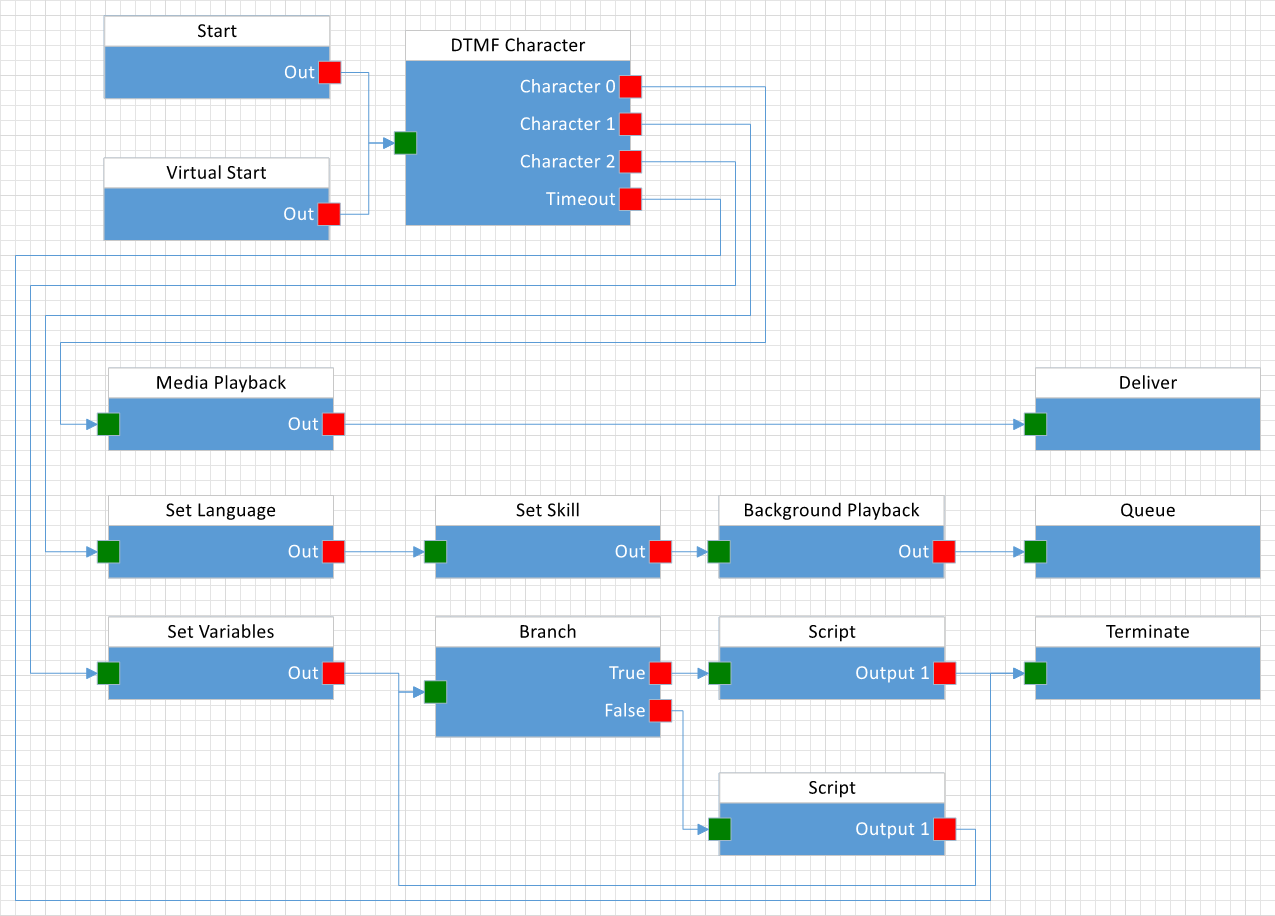
\includegraphics[width=\textwidth]{img/TestRouting.png}
	\caption[DSL-Modell für manuelle Tests]{Zu sehen ist das DSL-Modell, welches im Zuge von manuellen Tests zum Einsatz kommt.}
	\label{fig:TestRouting}
\end{figure}

\section{Metriken}
Bei der Umsetzung der DSL entstehen zwei Arten von Code. Die eine Art von Quellcode setzt das System um: Es handelt sich hierbei um den Quellcode, der den Editor und den Transformator implementiert. Die andere Art von Code ist der vom System generierte Code, also der CIL-Bytecode, der ein Routing implementiert. Beide Code-Sorten müssen eine hohe Qualität aufweisen, damit das System als Produkt zum einen einsatzfähig und zum anderen wartbar ist. Die im Folgenden beschriebenen Metriken vermessen und evaluieren diese beide Arten von Code. Berechnet wurden diese mit der Entwicklungsumgebung Visual Studio 2017 Ultimate. Zum Einsatz kommen hier die "Lines of Code", die zyklomatische Komplexität, auch als McCabe-Metrik bekannt, und der "Maintainability Index". Während die ersten beiden Metriken im Feld der Software-Architektur bekannt sind (unter anderem unter [CITATION] nachzulesen), ist der Maintainability Index ein Aggregat, welches verschiedene andere Werte in sich vereint. Es handelt sich um einen Ganzzahl-Wert von null bis 100, bei dem hohe Werte als positiv zu bewerten sind. Laut [CITATION 
\begin{comment}
https://blogs.msdn.microsoft.com/zainnab/2011/05/26/code-metrics-maintainability-index/ 
\end{comment}
] wird der Maintainability-Index folgendermaßen berechnet: 
\begin{dmath}
   \\max \left( 0, \left( 171 \\ - 5,2 * \log{\left(Halstead\ Volumen  \right)} \\ - 0,23 * \left( zyklomatische\ Komplexit\ddot{a}t \right) \\ - 16,2 * \log{\left(Lines\ of\ Code\right )} \\ \right) * 100 / 171 \right)
\end{dmath}
Das Halstead Volumen, beschrieben in [CITATION], ist ein weiteres Maß zur Einschätzung der Komplexität von Code. Code mit einem Maintainability Index zwischen 20 und 100 gilt als besonders wartbar. Ein Index unter 20 zeigt entweder eine mittelmäßige oder schlechte Wartbarkeit an. 

\subsection{Geschriebener Code}
In Tabelle \ref{tab:metrikenGeschriebenerCode} sind die gemessenen Metriken für den im Zuge der vorliegenden Arbeit händisch verfassten Code zu sehen.
\begin{center}
    \begin{tabular}{| l | l | l | l | l |}
    \hline
    Komponente & Namespace & LOC & zykl. Kompl. & Maint. Index\\ \hline
    Semantisches Modell & ConversationFlow.Core & 183 & 141 & 92 \\ \hline
    Editor & ConversationFlow.UI & 465 & 2818 & 78 \\ \hline
    Transformator & ConversationFlow.Generation & 730 & 299 & 76 \\ \hline
    Validator & ConversationFlow.Validation & 186 & 112 & 85 \\ \hline
    \end{tabular}
    \label{tab:metrikenGeschriebenerCode}
\end{center}
Das semantische Modell weist die niedrigste Komplexität auf. Dies ist nicht überraschend, da es sich um eine fast reine Datenstruktur handelt, die wenig programmatisches Verhalten aufweist. An zweiter Stelle kommt die Komponente der Modell-Validierung. Komplexe Strukturen, welche die Metriken negativ beeinflussen, konnten hier vermieden werden, da die meiste Arbeit, die solche Strukturen erfordert, an andere Komponenten ausgelagert wird. Eine deutlich höhere Komplexität weißt der Editor auf. Die Werte für diese Komponente lassen sich damit begründen, dass automatisch generierter Code des Devexpress-Framework in diesem Namespace enthalten ist. Devexpress benutzt einen sogenannten Component Designer, welcher "Boilerplate"-Code zum Erstellen von Windows Forms-Komponenten automatisch generiert. Dieser Code ist lang und dank seines Umfangs komplex. Zwar fallen die hohen Werte der Metriken dadurch auf, sind aber irrelevant, da der vom Component Designer generierte Code nicht von Hand lesbar oder editierbar sein soll und damit nicht die Komplexität des System widerspiegelt. Die laut dem Maintainability Index komplexeste Komponente ist der Transformator. 
\subsection{Generierter Code}
TODO

\section{Performanz}
TODO

\subsection{Geschriebener Code}
TODO

\subsection{Generierter Code}
TODO

\chapter{Zusammenfassung und Ausblick}
Für den Produktivbetrieb als Teil des Produktes MyCC braucht die vorliegend implementierte DSL noch Anpassungen, vor allem im Bereich der umliegenden Infrastruktur. 
Dennoch ist die DSL bereits weit fortgeschritten. Der Entwurf der Sprache geht mit der Abdeckung der eingangs erwähnten Anforderungen einen großen Schritt auf die Produkt-Vision einer freien Konversationsroutingmodellierung durch den Benutzer zu. Diesem Entwurf folgt die Implementierung von drei Komponenten, die für eine Umsetzung der DSL nötig sind. Eine dieser Komponenten ist der Editor, der dank flexibler MVVM-Struktur ein funktionsfähiger Prototyp der finalen Benutzeroberfläche ist. Eine weitere ist der Transformator, der sich die Roslyn-API zu Nutze macht, um lauffähige CIL-Syntax zu generieren und zu kompilieren, um anschließend eine betriebsfähige Assembly an die Routing Engine auszuliefern. Die dritte Komponente ist die  Modell-Validierung, welche dem Benutzer während der Modellierung laufend Feedback gibt und dabei hilft, etwaige Fehlerzustände frühzeitig zu beheben. 
\newline
Zusammen machen es diese drei Komponenten bereits möglich, erste funktionstüchtige Konversationsroutings zu spezifizieren. Wie manuelle und automatisierte Tests zeigen, können diese auch erfolgreich ausgeführt werden. Neben den funktionalen Anforderungen erweist sich das System außerdem als ausreichend performant. Die Implementierung stützt sich dabei auf gradlinigen Code, welcher die Wartbarkeit des Systems auch für zukünftige Erweiterungen sicher stellt. 
\newline
Für solche bietet das System auch in Zukunft Raum: So ist unter anderem die Unterstützung von anderen Kontaktmöglichkeiten wie Emails oder Web Chats für Konversationsroutings in Planung. Zusätzlich kann der eigentliche Umgang mit einem Kontakt erweitert werden, zum Beispiel indem dem Benutzer die Möglichkeit gegeben wird, nach der Zustellung zu einem Agenten weiterhin mit dem Anruf zu interagieren. Denkbar ist dies durch die Einführung von Event-Instruktionen, welche ausgeführt werden, wenn der Agent den Ruf annimmt oder anderweitige Ereignisse auftreten. Nicht zuletzt das Repertoire an Instruktionen bietet weiteren Implementierungsspielraum: Instruktionen, welche das Anreichern von Anrufen mit Anrufer-spezifischen Daten erlauben, böten dem Benutzer einen erheblichen Mehrwert. Alles in Allem bietet die umgesetzte DSL eine erste Implementierung mit Erweiterungspotential und damit eine solide Basis zur weiteren 
Umsetzung eines integralen Features von MyContactCenter.
% ...
%--------------------------------------------------------------------------
\backmatter                        		% Anhang
%-------------------------------------------------------------------------
\bibliographystyle{geralpha}			% Literaturverzeichnis
\bibliography{literatur}     			% BibTeX-File literatur.bib
%--------------------------------------------------------------------------
\printindex 							% Index (optional)
%--------------------------------------------------------------------------
%\begin{appendix}						% Anhänge sind i.d.R. optional
%   \include{chapters/Glossar}			% Glossar   
%   \chapter{Erkl�rung der Kandidatin / des Kandidaten}

\begin{description}[$\Box$~]
\item[$\Box$] Die Arbeit habe ich selbstst�ndig verfasst und keine anderen als die angegebenen Quellen- und Hilfsmittel verwendet.\\

\item[$\Box$] Die Arbeit wurde als Gruppenarbeit angefertigt. Meine eigene Leistung ist\\
...\\

Diesen Teil habe ich selbstst�ndig verfasst und keine anderen als die angegebenen Quellen und Hilfsmittel verwendet. \\

Namen der Mitverfasser: ...

\end{description}

\vspace{2cm}

\begin{minipage}[t]{3cm}
\rule{3cm}{0.5pt}
Datum
\end{minipage}
\hfill
\begin{minipage}[t]{9cm}
\rule{9cm}{0.5pt}
Unterschrift der Kandidatin / des Kandidaten
\end{minipage}	% Selbstständigkeitserklärung
%\end{appendix}

\end{document}
